\subsection{\textit{RNNIP} Tagger}

\label{sec:rnn-result-rnn}

To understand the performance of the \textit{RNNIP} algorithm, the $b$-tagging efficiency and background rejection (1 / background efficiency) are examined inclusively and as a function of the jet $\pt$. As the \textit{RNNIP} has a four-class output, several of these outputs are combined into the following discriminant function:
\begin{equation}
D_{\mathrm{RNN}} = \ln \frac{p_{b}}{f_c p_c + (1-f_c) p_l}
\end{equation}
where $f_c$ is a parameter representing the $c$-jet fraction, which can be used change the relative importance of $c$-jet and light-jet rejection by the discriminant.  This parameter is fixed at $f_c=0.07$, which is close to the 8\% $c$-jet fraction present in the $t\bar{t}$ training sample. The tau output $p_\tau$ is ignored.

Inclusive background rejection versus signal efficiency curves are produced by scanning a minimum threshold on $D_{\mathrm{RNN}}$ and computing background rejection and signal efficiency at each threshold. These curves can be found in Figure~\ref{fig:ROC}, for a background of light jets and a background of $c$-jets separately.  Curves are also presented for \textit{IP3D}, \textit{SV1}, and \textit{MV2}. One can see that the \textit{RNNIP} outperforms other low-level taggers like \textit{IP3D} and \textit{SV1}. As the \textit{RNNIP} tagger operates directly on tracks, utilizing both impact parameter and kinematic information and taking into account track-to-track correlations, it is not surprising that it outperforms the \textit{IP3D} algorithm.  However, the performance is not as strong as that of \textit{MV2}, which is expected because \textit{MV2} combines information from several low-level tagging algorithms, utilizing more information than is being fed to the RNN. To understand the origin of the performance gain of \textit{RNNIP} compared to \textit{IP3D}, the ROC curves of the RNN taggers using only the same inputs as \textit{IP3D} and using all track features including $\ptfrac$ and $drtj$ are shown Fig.\ref{fig:IP3D-RNN}. The adoption of RNN algorithm and the inclusion of more track variables both boost the light jet and $c$-jet rejections.

\begin{figure}[htbp]
  \centering
 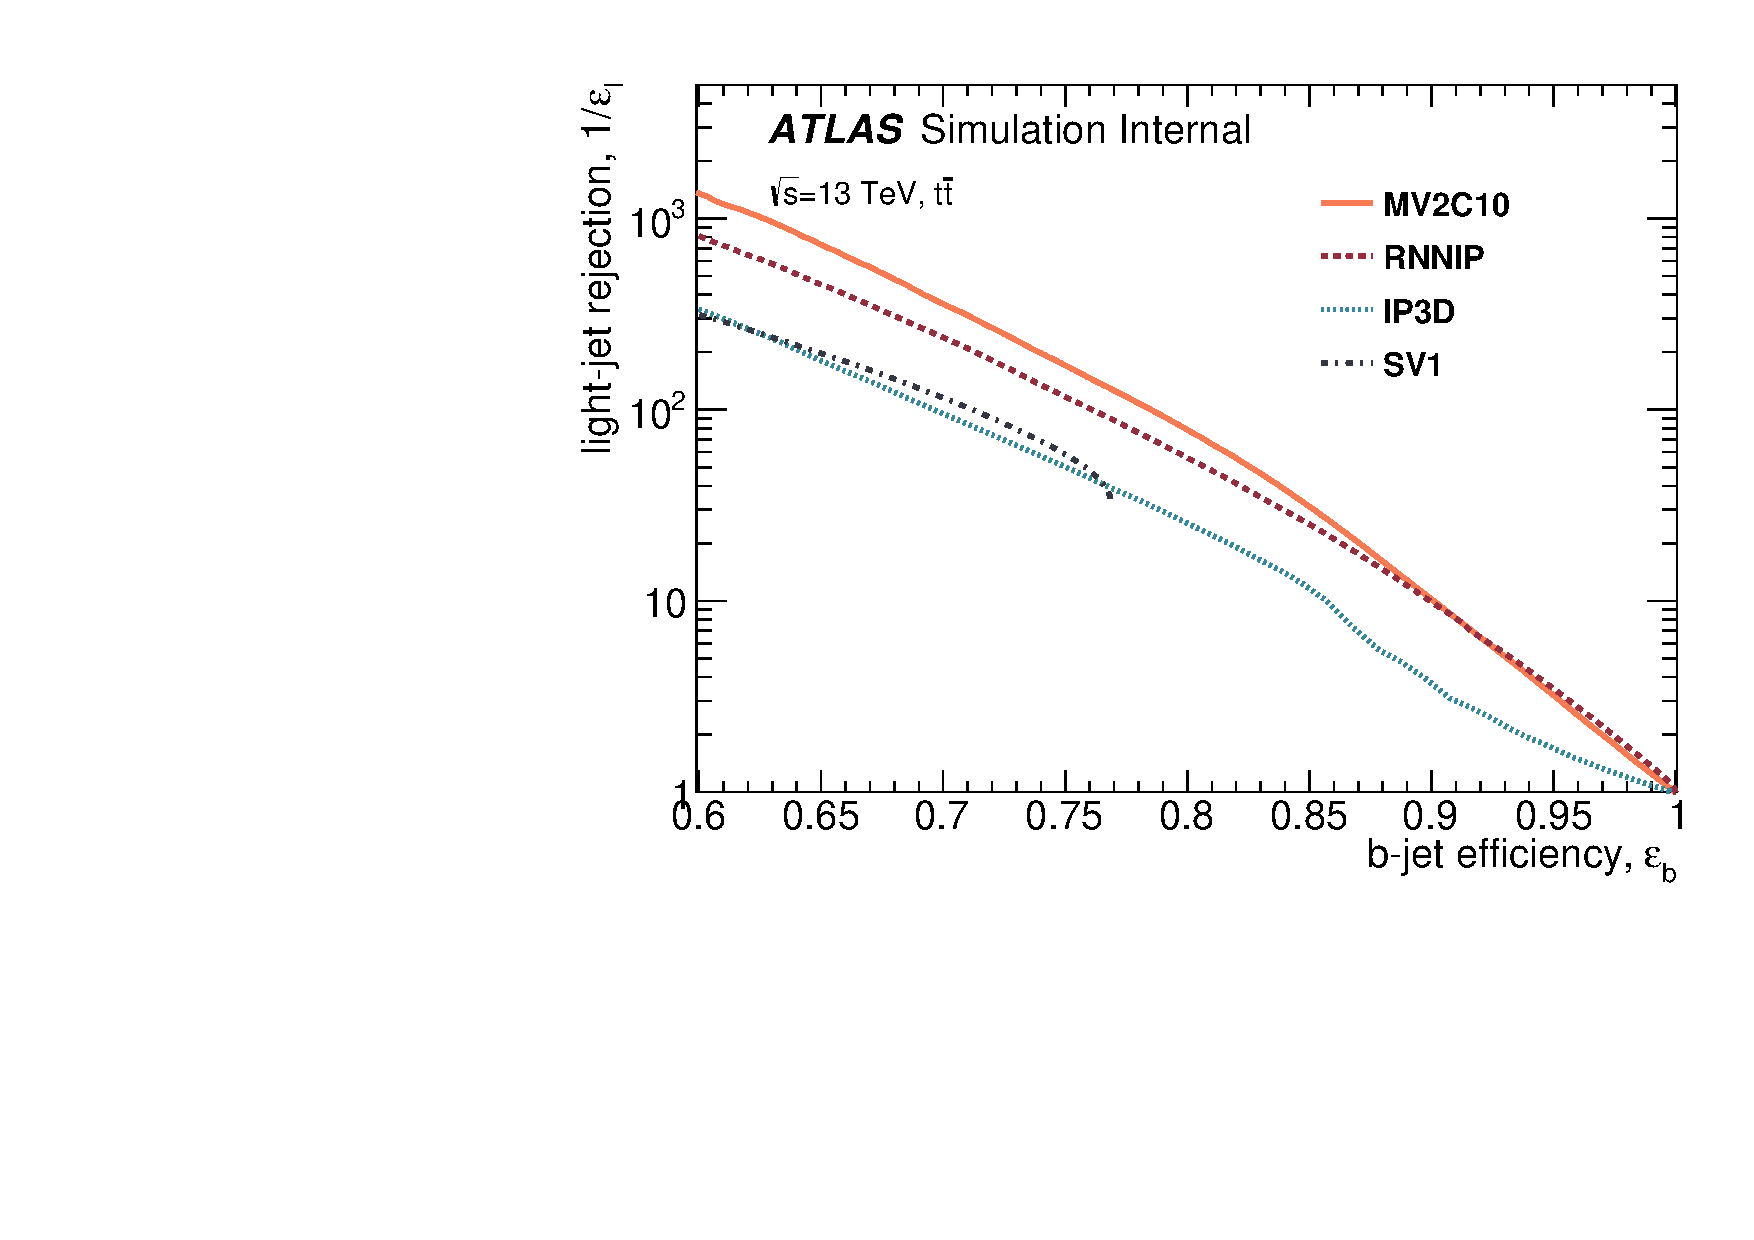
\includegraphics[width=0.48\textwidth]{figures/RNN/BL_ROC.pdf}
 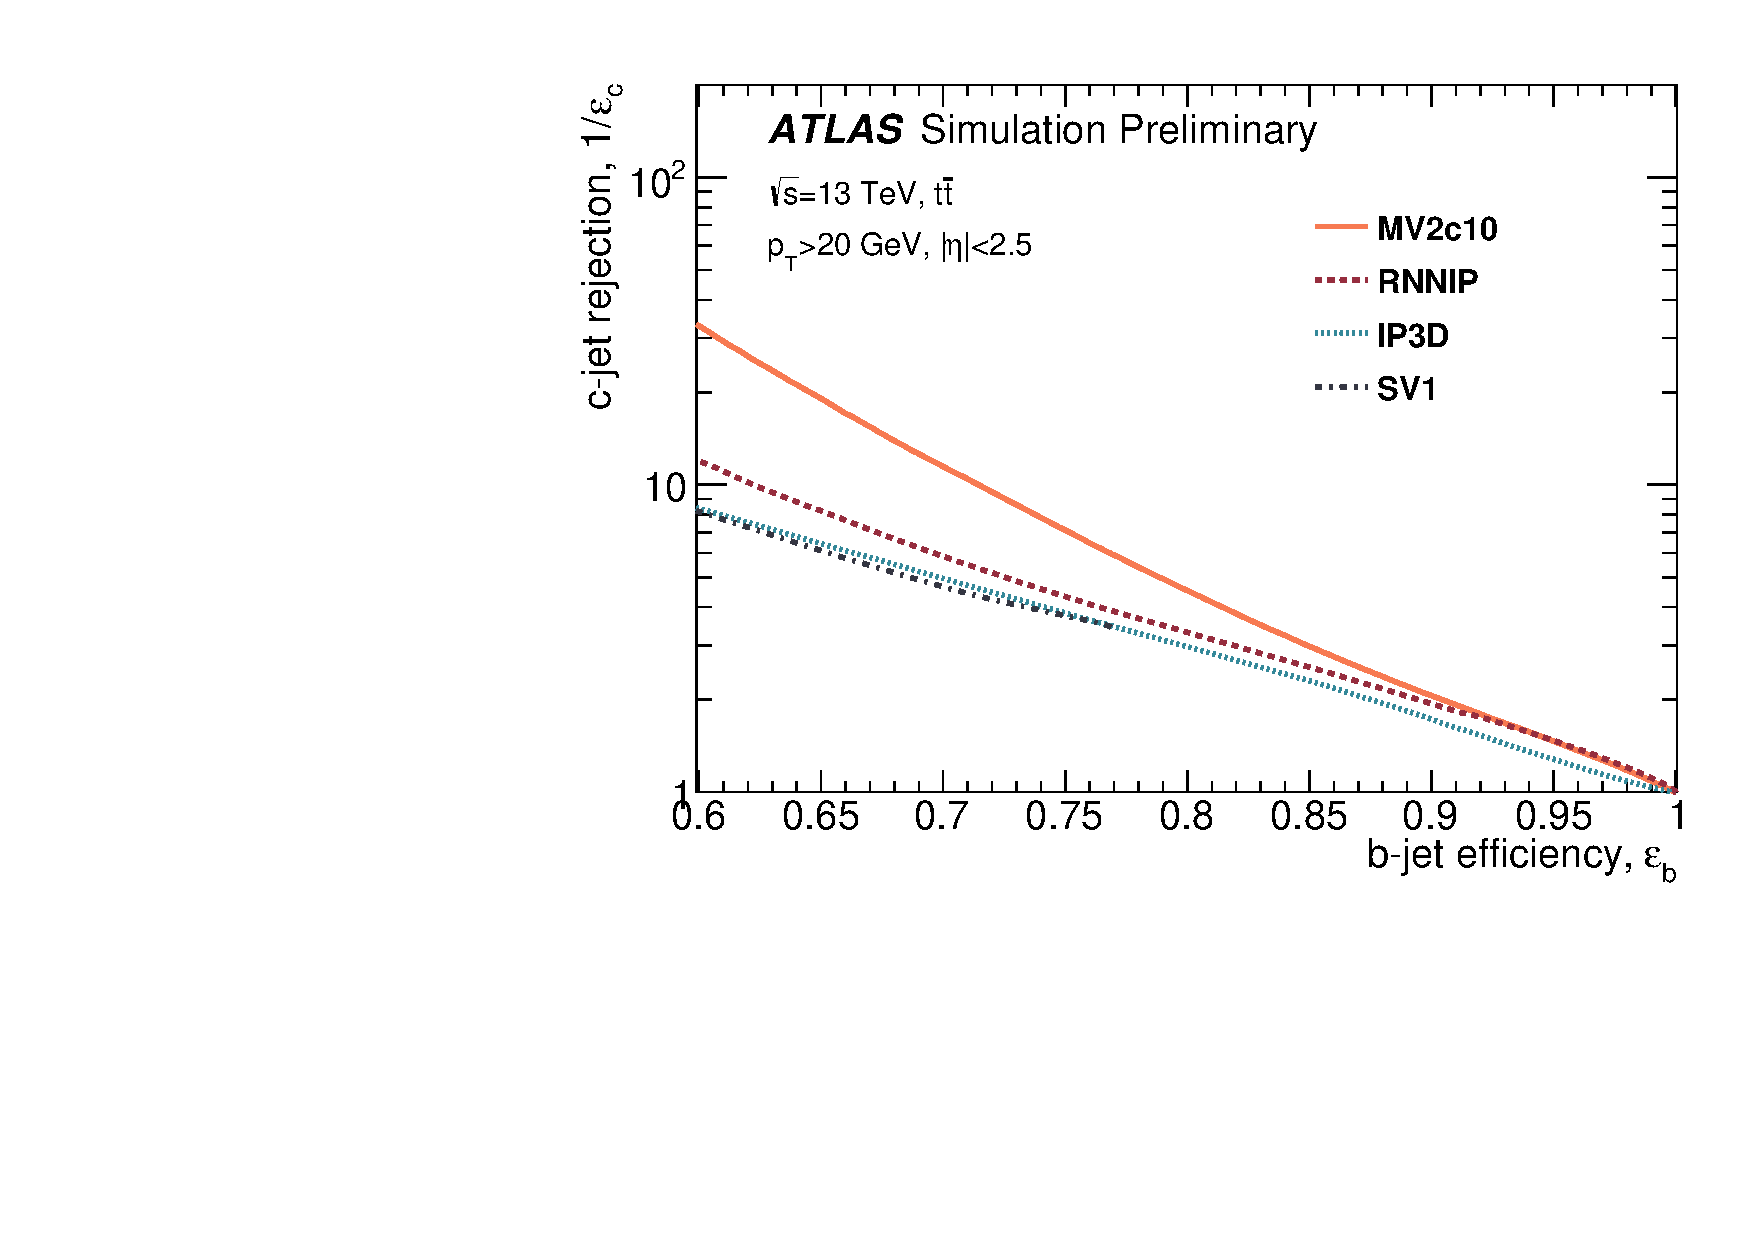
\includegraphics[width=0.48\textwidth]{figures/RNN//BC_ROC.pdf}
\caption{The light-jet (left) and $c$-jet (right) rejection versus $b$-tagging efficiency for jets with $p_T > 20$ GeV and $|\eta|<2.5$. The statistical error on the curve is less than 3\%.}
  \label{fig:ROC}
\end{figure}

\begin{figure}[htbp]
  \centering
 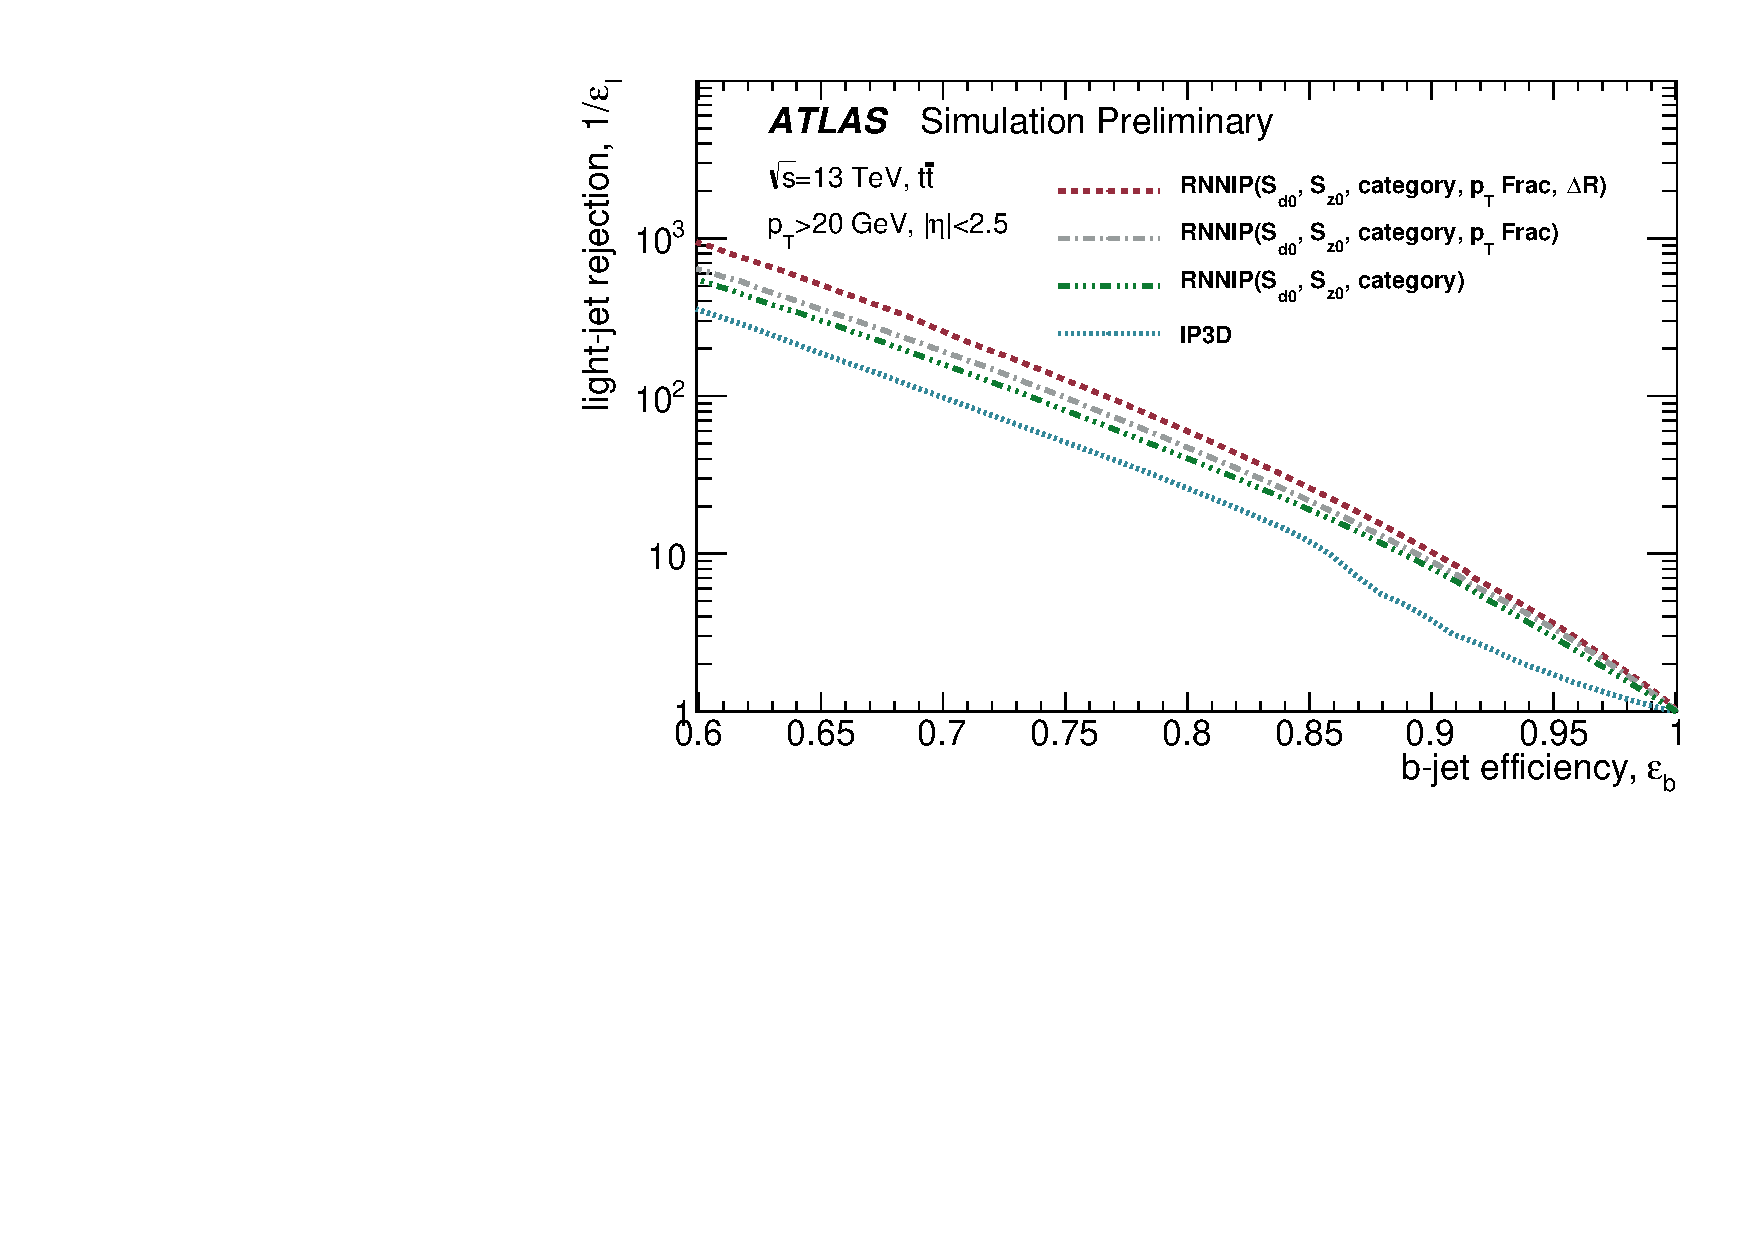
\includegraphics[width=0.48\textwidth]{figures/RNN/BL_ROC_RNNComp.pdf}
 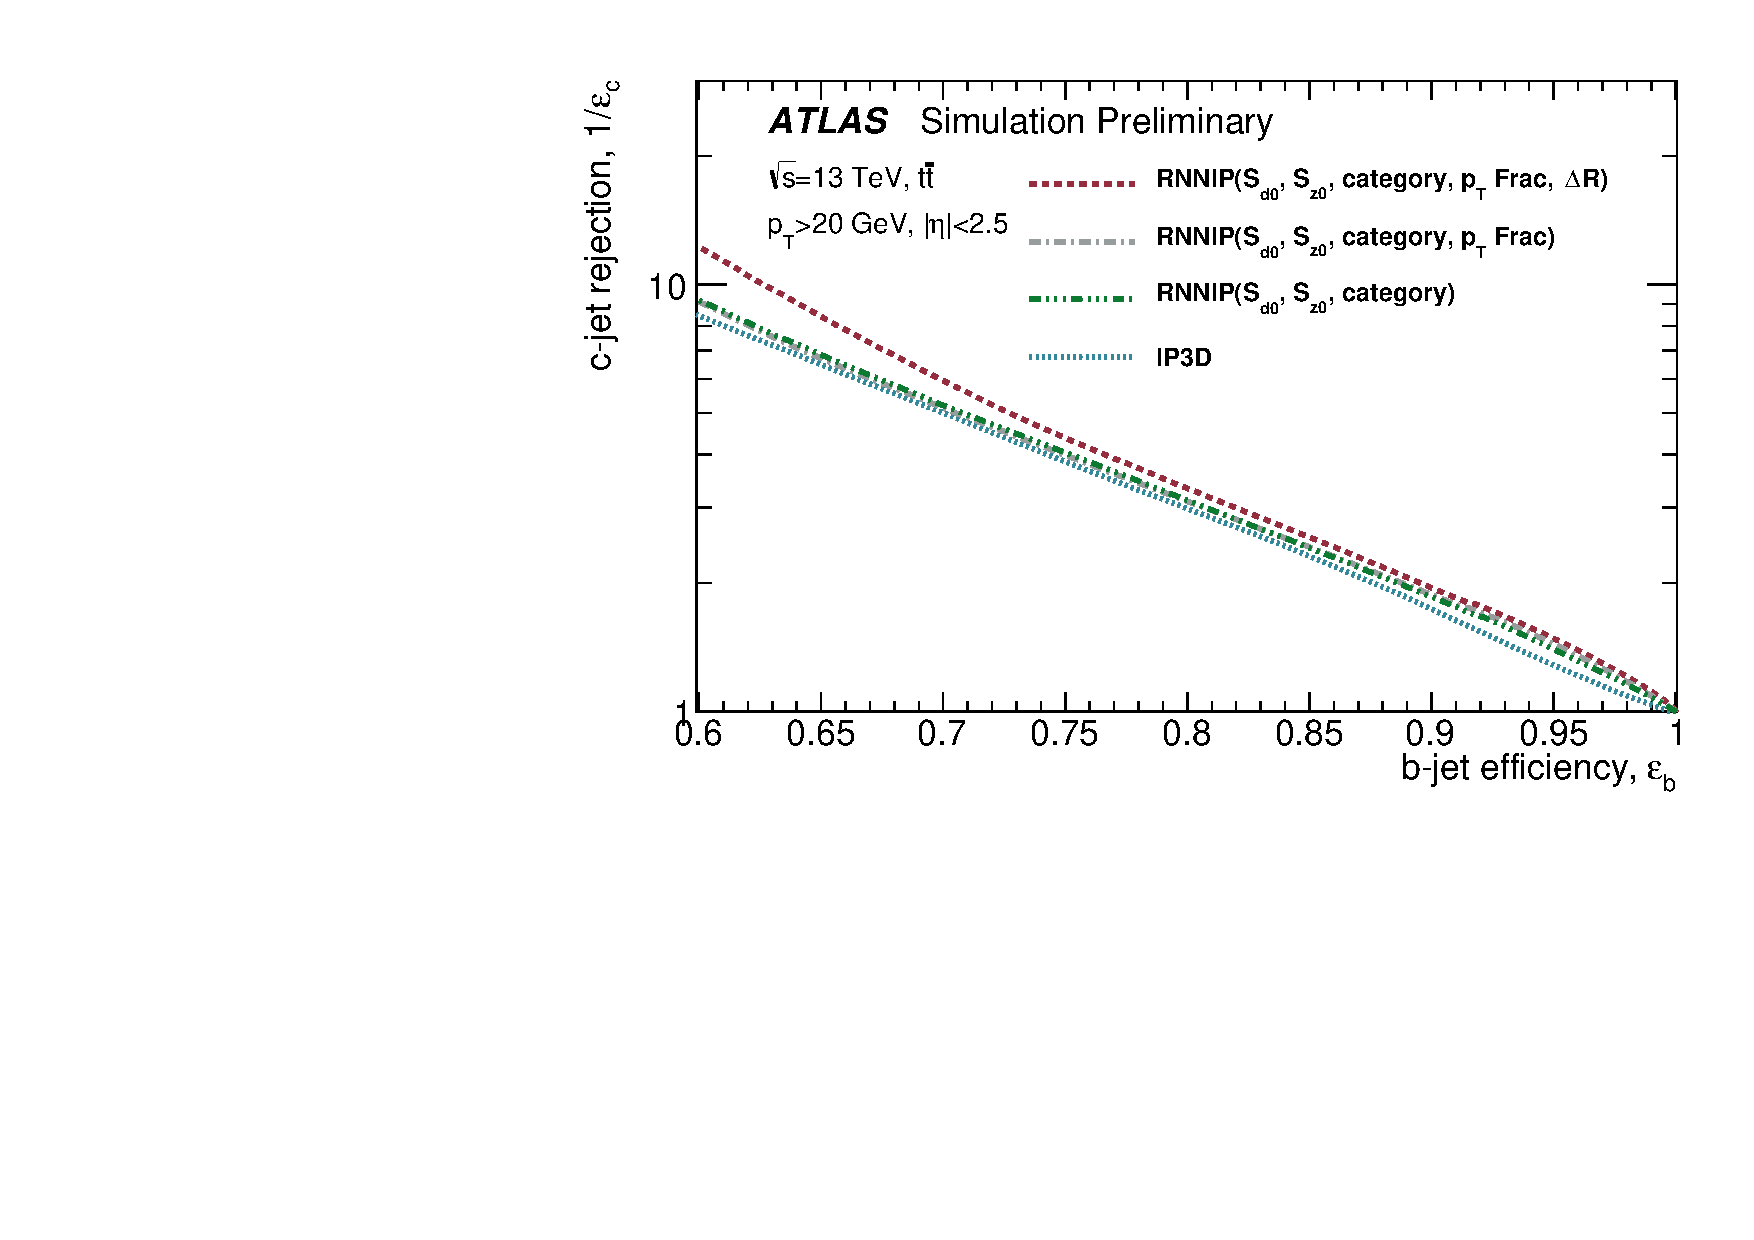
\includegraphics[width=0.48\textwidth]{figures/RNN//BC_ROC_RNNComp.pdf}
 \caption{The light-jet (left) and c-jet (right) rejection versus b-tagging efficiency for jets with $\pt > 20 \gev$ and $|\eta|$<2.5, for RNNs trained using various sets of input variables, and for \textit{IP3D}. The \textit{RNNIP} without $\ptfrac$ and $drtj$ uses only the inputs available to \textit{IP3D}.}
  \label{fig:IP3D-RNN}
\end{figure}


In order to gain insights of how the tagging performance depends on jet kinematics, the $b$-tagging efficiency versus jet $p_T$ is shown in Figure~\ref{fig:fixed_eff_pt}. To isolate the effect of a changing $b$-tagging efficiency from that of the changing light-jet and $c$-jet rejection rejection, a flat-efficiency 70\% WP is examined.  In this case, all taggers will have a 70\% efficiency across $p_T$, and only the rejection is varying.  The light- and $c$-jet rejection as a function of jet $p_T$ can be seen in Figure~\ref{fig:flat_rej_pt}.  One can see that the \textit{RNNIP} outperforms \textit{IP3D} and \textit{SV1} in terms of light-jet rejection across the $p_T$ range, and outperforms \textit{IP3D} in terms of charm rejection.

\begin{figure}[htbp]
  \centering
 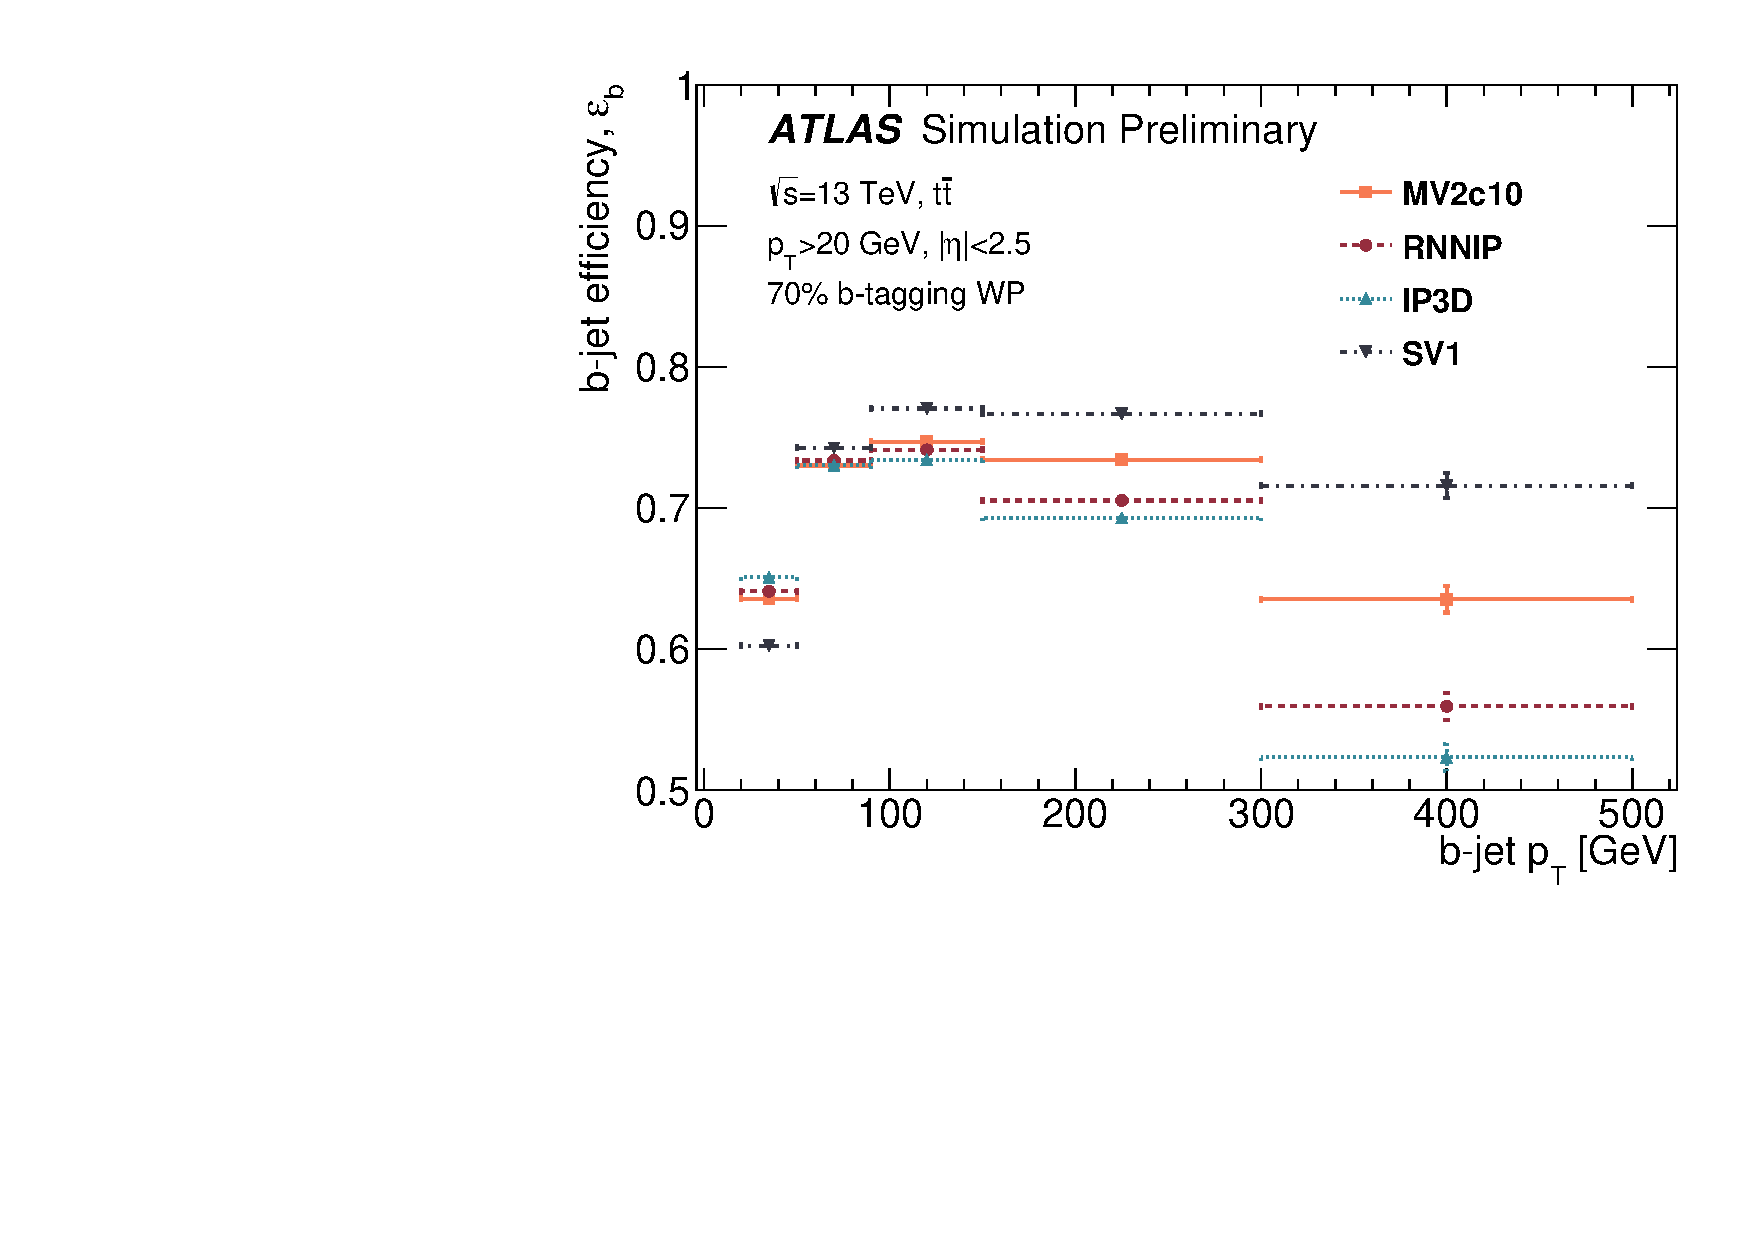
\includegraphics[width=0.48\textwidth]{figures/RNN/BEff_FixWP70.pdf}
\caption{$b$-tagging efficiency for a 70\% WP cut versus jet $p_T$. }
  \label{fig:fixed_eff_pt}
\end{figure}

\begin{figure}[htbp]
  \centering
 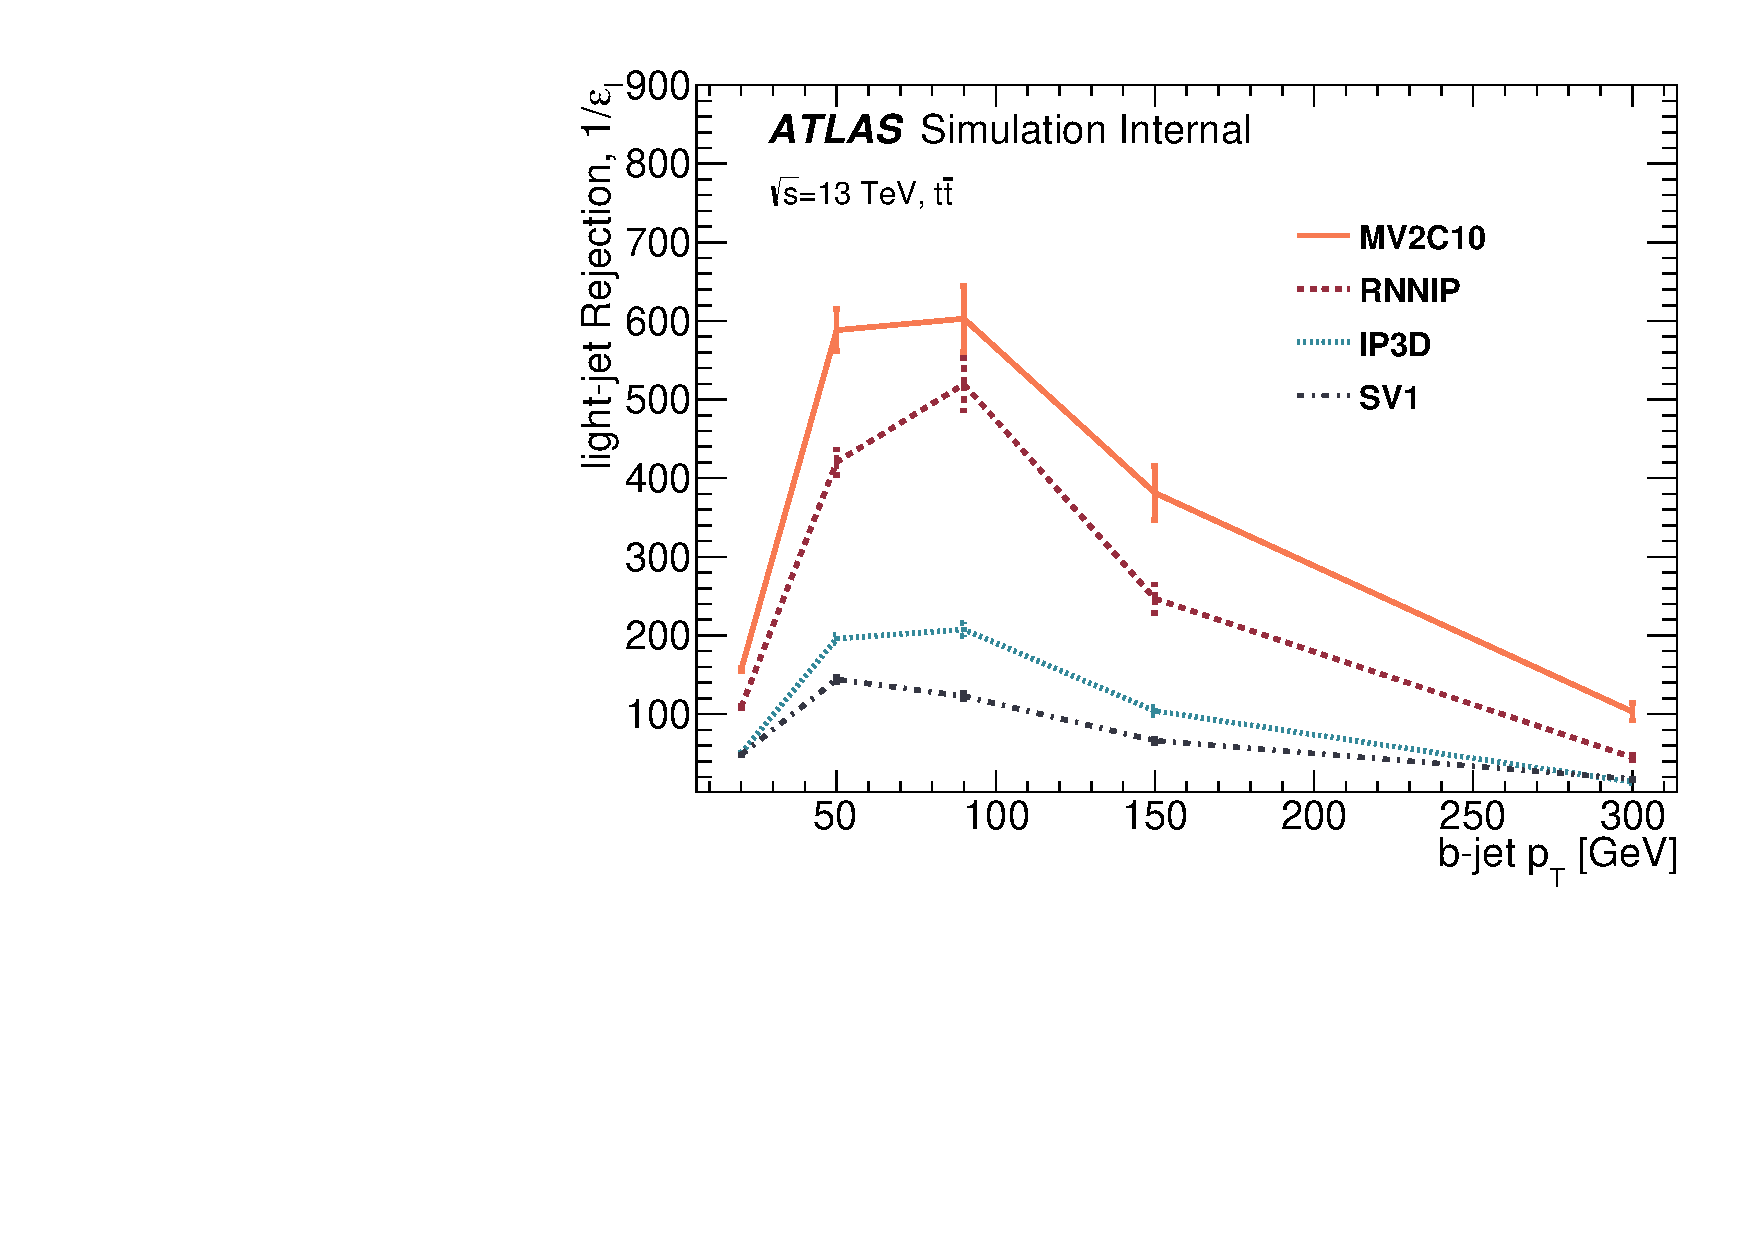
\includegraphics[width=0.48\textwidth]{figures/RNN/LRej_FlatEff.pdf}
  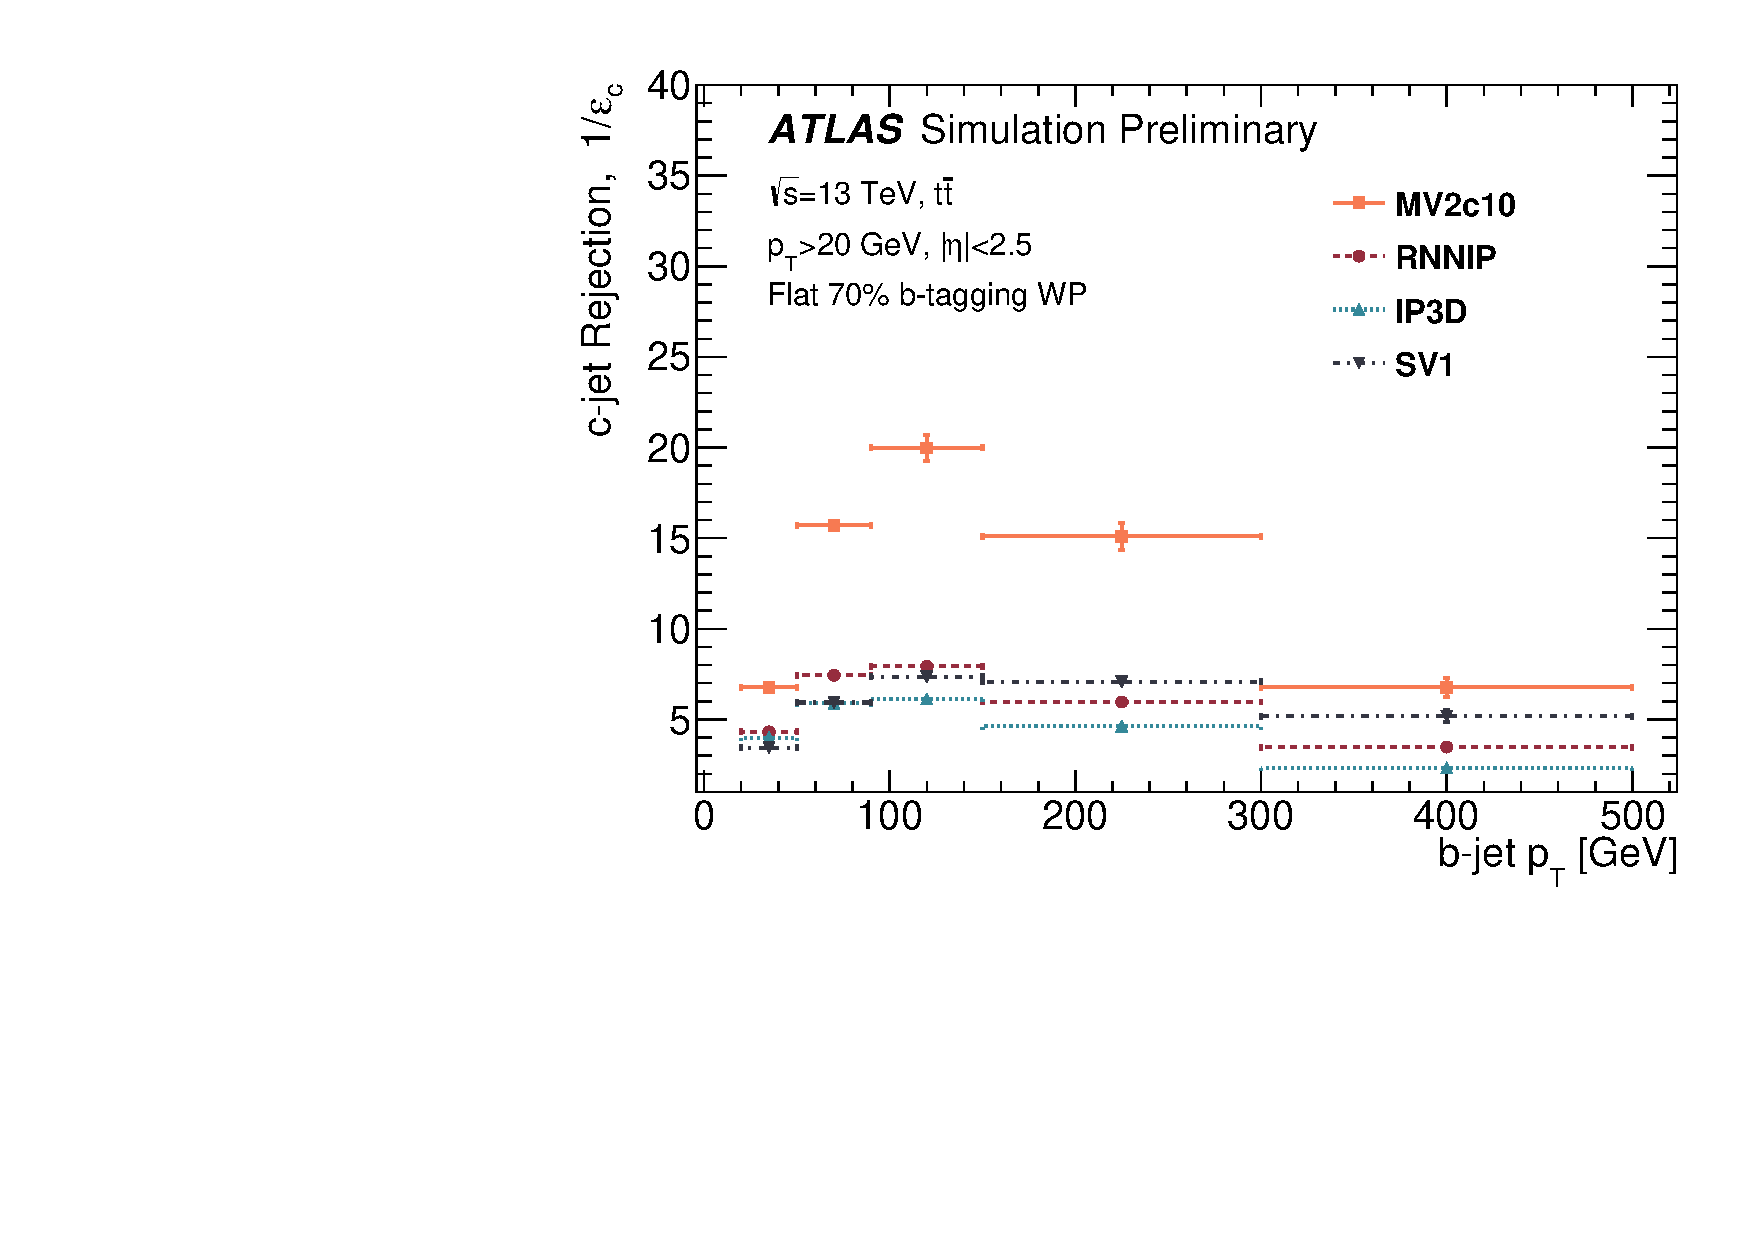
\includegraphics[width=0.48\textwidth]{figures/RNN/CRej_FlatEff.pdf}
\caption{Light jet rejection (left) and $c$-jet rejection (right) at flat $b$-tagging efficiency of 70\% versus jet $p_T$.}
  \label{fig:flat_rej_pt}
\end{figure}

%While the power of the RNN approach applied directly on track related variables can be seen from the efficiency and rejection curves, the source of this performance is difficult to pinpoint as this information is carried in the learned weights of the network and is not easy to interpret.  


The power of the RNN approach, which can be inferred directly from the ROC curves, is due to the deep network’s ability to build complex, non-linear, hierarchical, internal representations, and it is therefore hard to assign the performance increase to any specific input variable.
However, one can examine how the RNN discriminant $D_{\mathrm{RNN}}$ depends on the inputs to the network by examining the Pearson linear correlation coefficient, $\rho$ between the per track input variables and $D_{\mathrm{RNN}}$.  This can be seen in Figure~\ref{fig:input_output_corrs}.  The strongest correlation is the $S_{d_0}$, especially for the first  $\sim8$ tracks in the sequence.  This may be related to the typical charged particle multiplicity expected in a $b$-jet. $S_{z_0}$ is the second most correlated variable. There is a small negative correlation with the $p_T^{\textrm{frac}}$, especially for tracks later in the sequence, which may be related to the harder fragmentation of $b$-quarks compared to lighter quarks, leading to an expectation of only a small number of high $p_T^{\textrm{frac}}$ tracks. Finally there is a small negative correlation with $\Delta R$, indicating that tracks far from the jet axis are less likely inside of $b$-jets where most tracks from a high momentum $b$-hadron are collimated.

\begin{figure}[htbp]
  \centering
 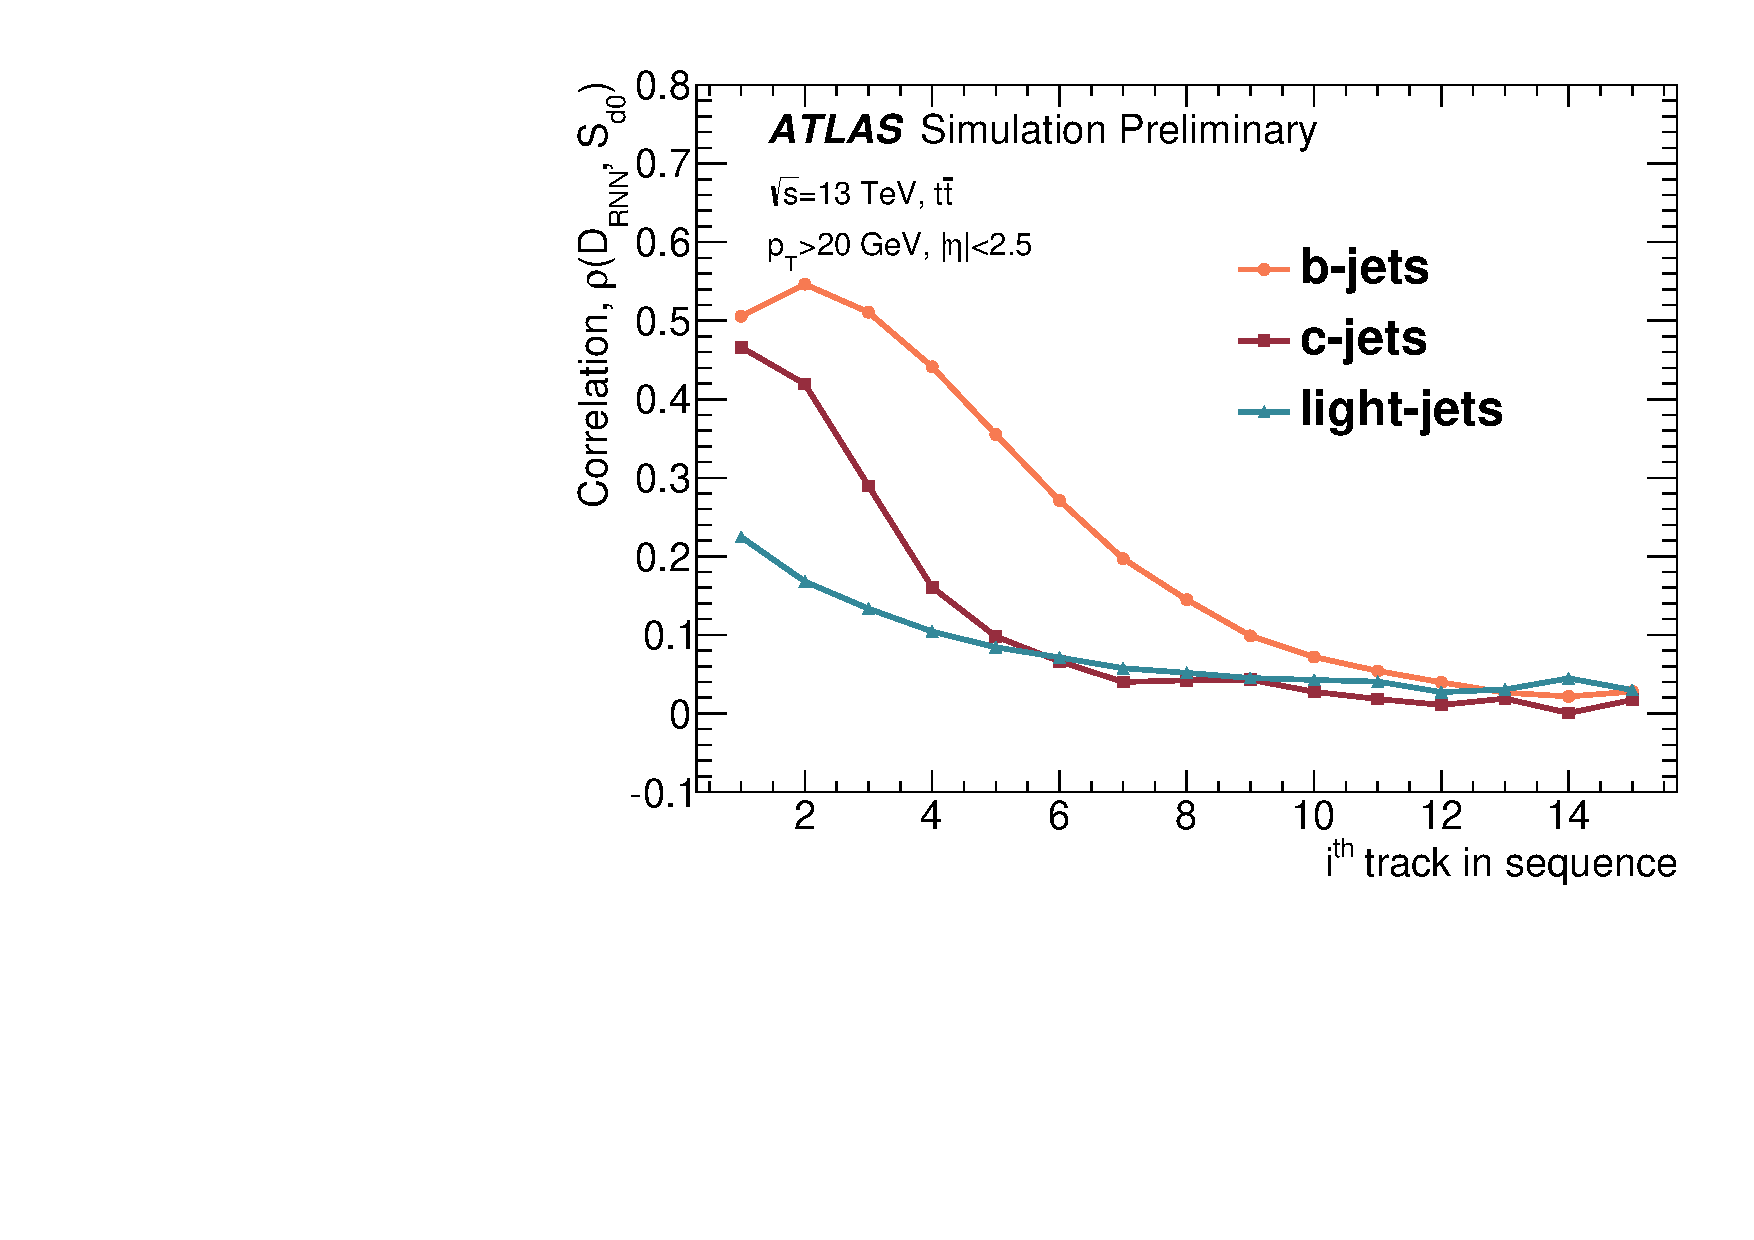
\includegraphics[width=0.48\textwidth]{figures/RNN/Corr_Sd0.pdf}
 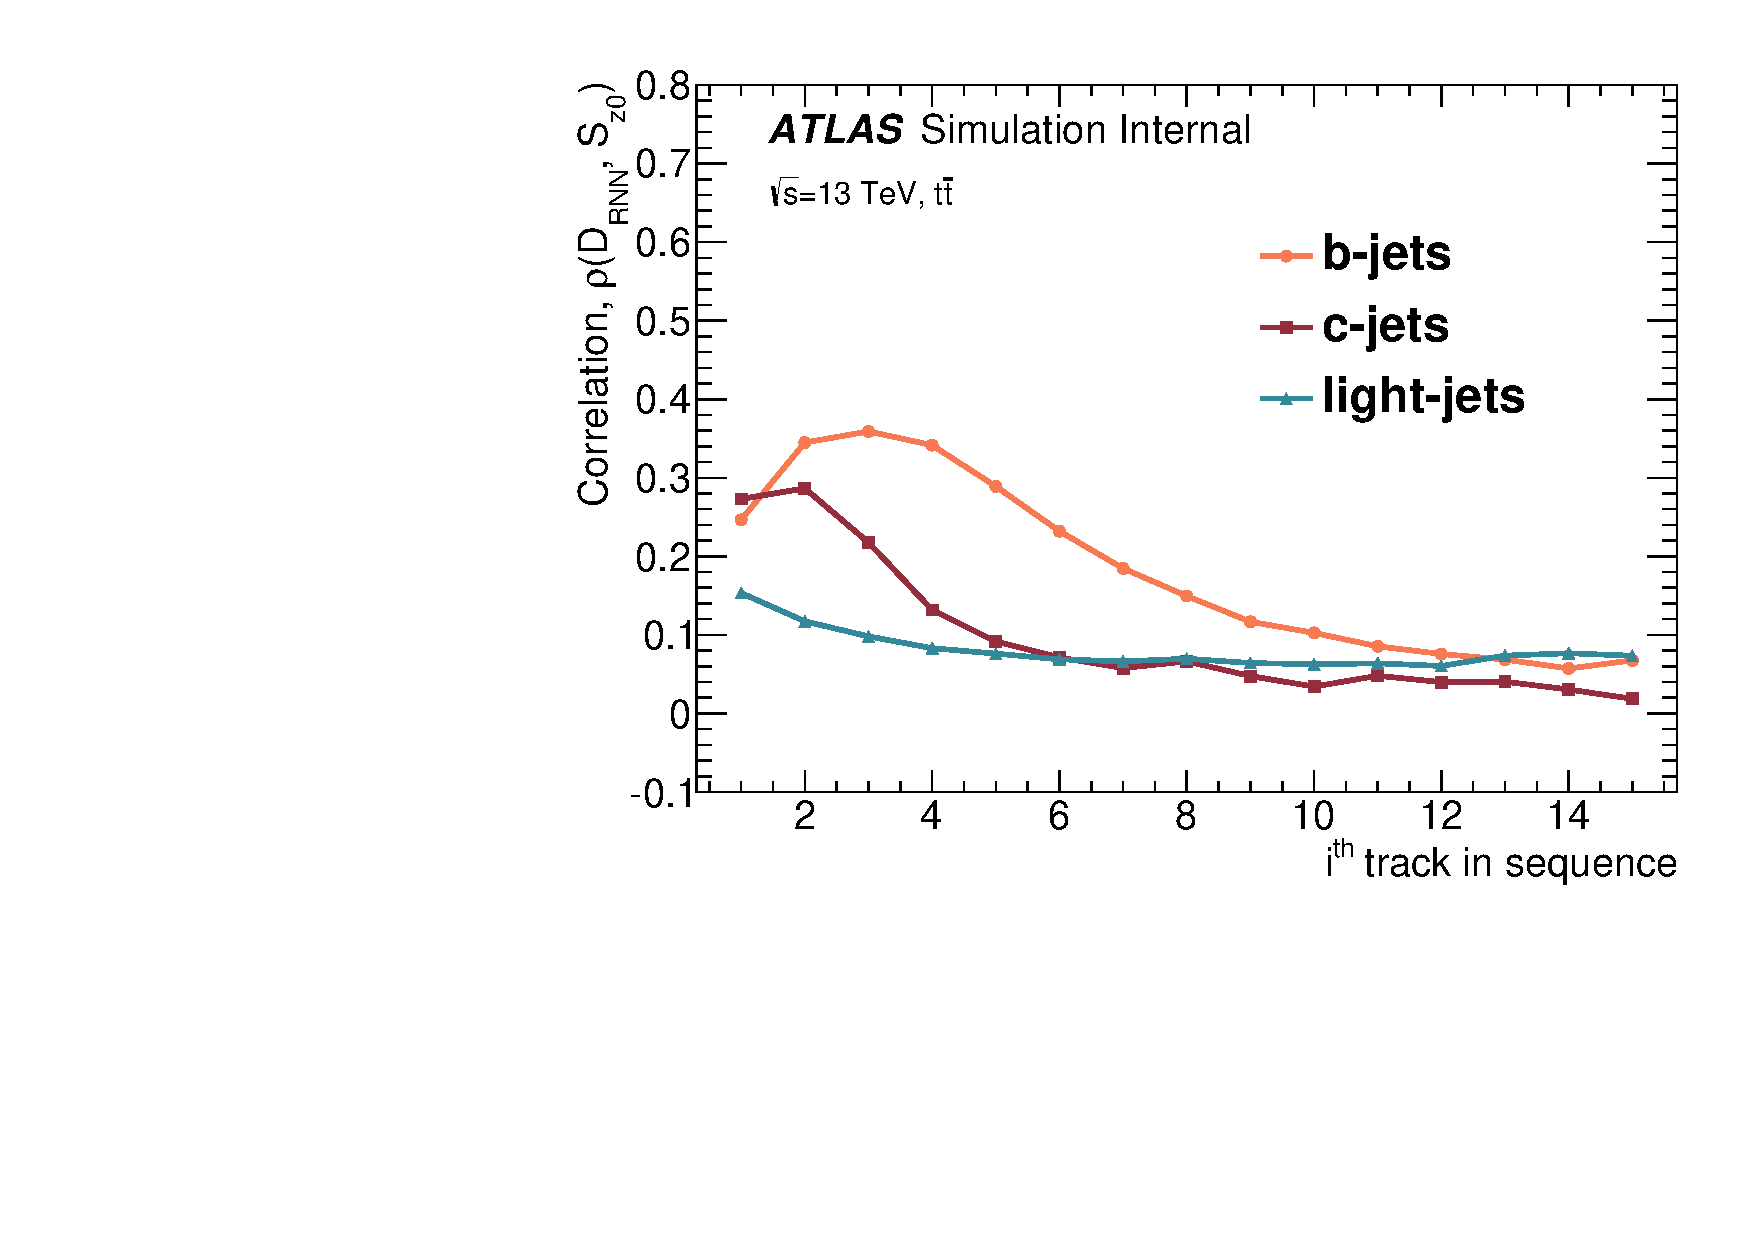
\includegraphics[width=0.48\textwidth]{figures/RNN/Corr_Sz0.pdf}
 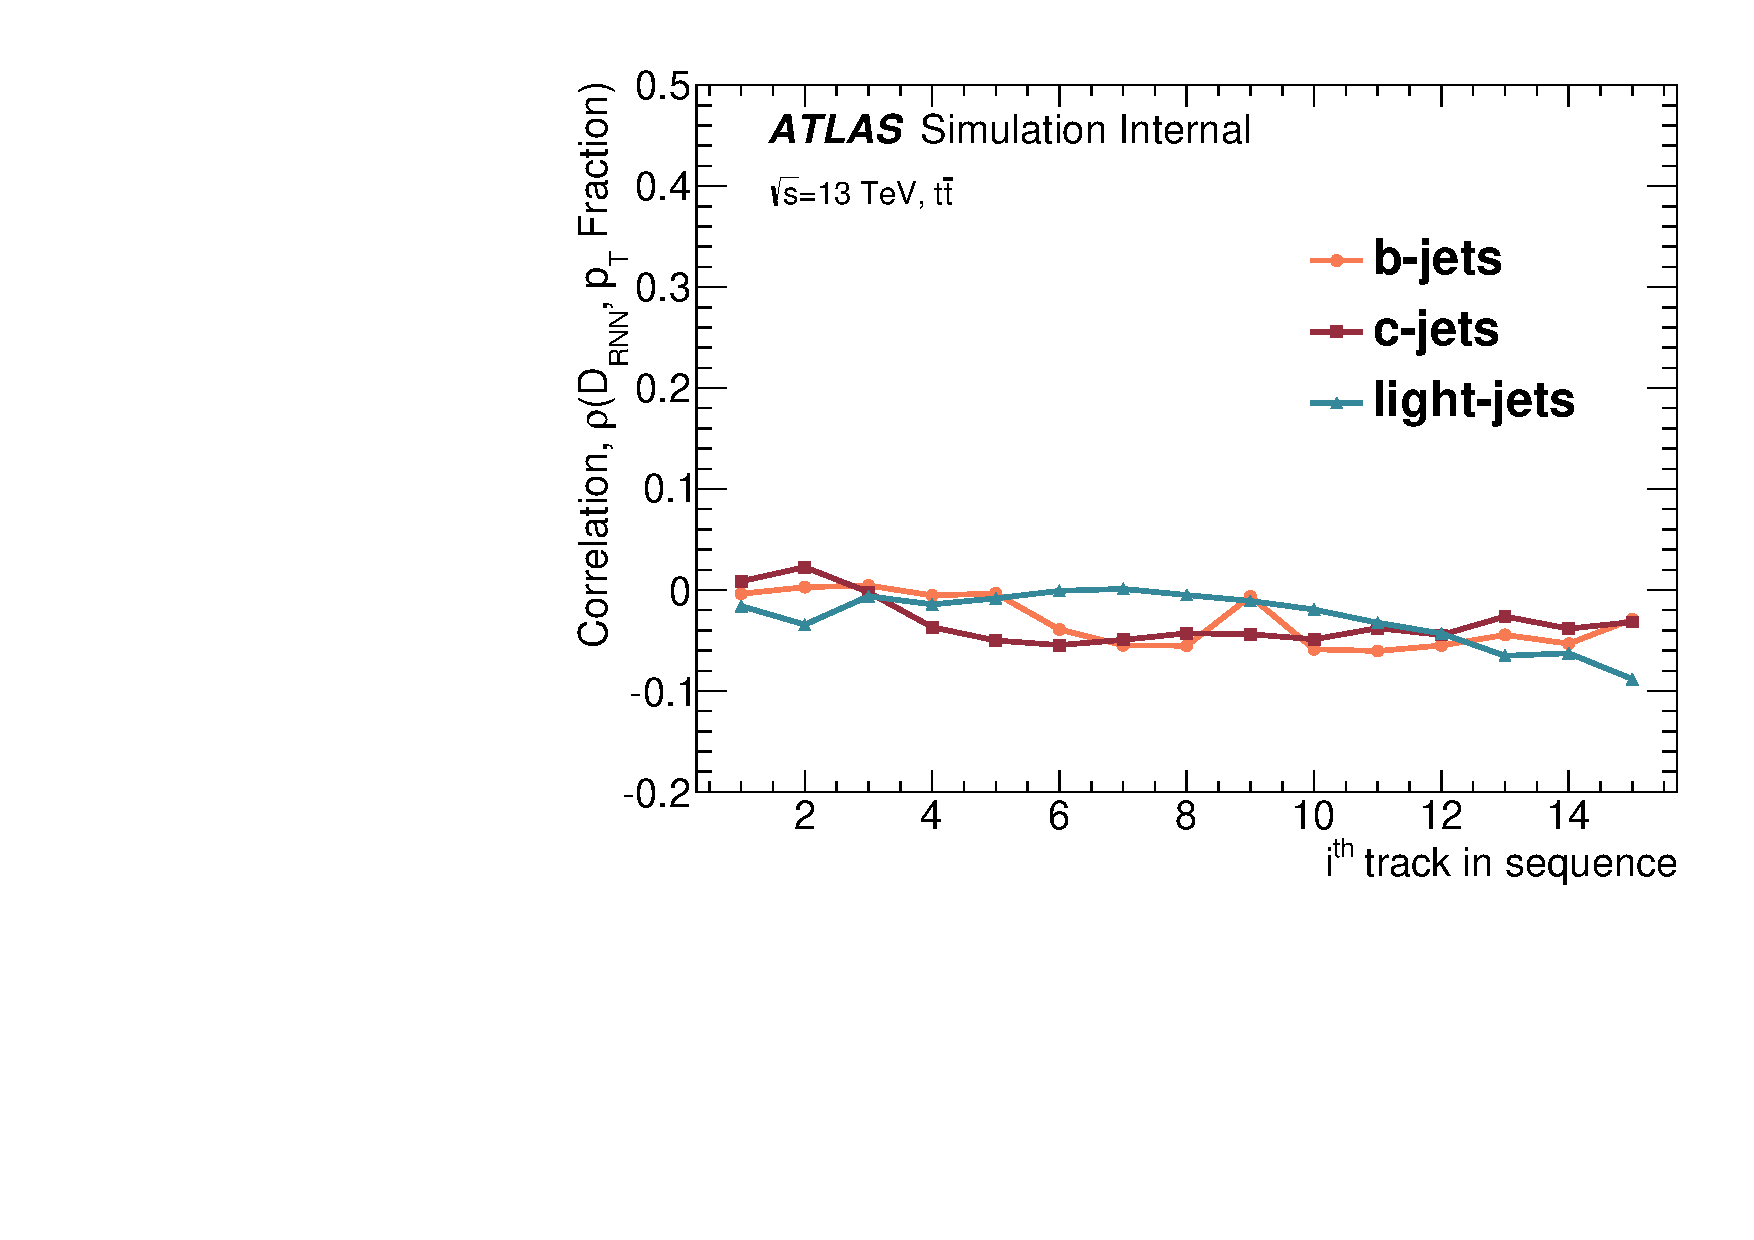
\includegraphics[width=0.48\textwidth]{figures/RNN/Corr_pTFrac.pdf}
 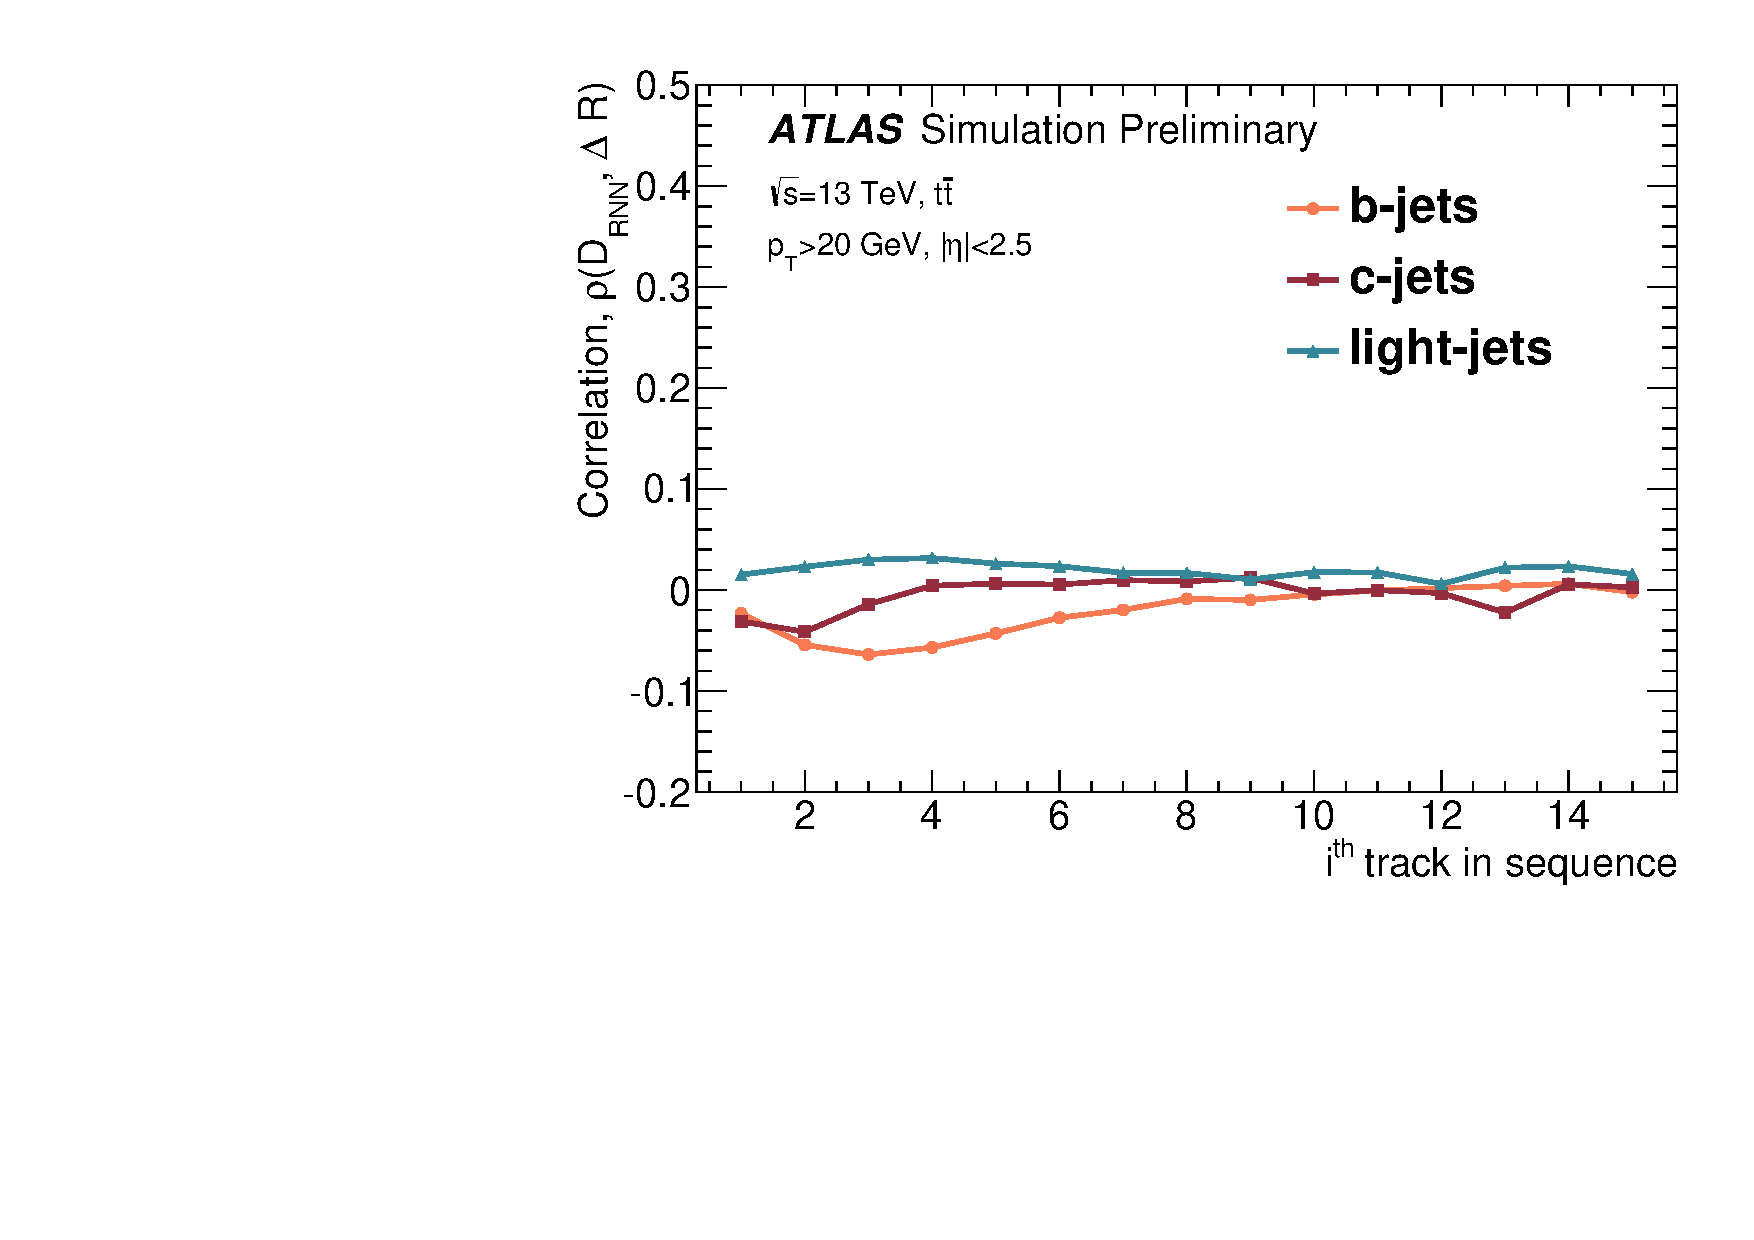
\includegraphics[width=0.48\textwidth]{figures/RNN/Corr_DeltaR.pdf}

\caption{Correlations of per track input variables $S_{d_0}$ (top left), $S_{z_0}$ (top right), $p_T^{\textrm{frac}}$ (bottom left), and $\Delta R$, with the RNN score $D_{\mathrm{RNN}}$.}
  \label{fig:input_output_corrs}
\end{figure}


\subsection{Combination with ATLAS Taggers}

\label{sec:rnn-result-combination}
The ultimate goal of the study is to improve the $b$-tagging performance. One possible critique of the \textit{RNNIP} Tagger is that the correlation of the track parameters stem from the fact that there exist secondary vertices in the $b$-hadron decay chain. If such correlation is already captured by other taggers such as \textit{SV1}, the overall performance of the combined tagger may not be improved. As shown in Fig.\ref{fig:combtagger}, combined with other baseline taggers of \textit{MV2} and another newly designed soft muon tagger which seeks to incorporate the muon information from the semi-leptonic decays, the RNN IP tagger does provide orthogonal information and boosts the combined algorithm performance for $c$-jet rejection, in high $b$-tagging efficiency regime and high $\pt$ regime. 


\begin{figure}[htbp]
  \centering
 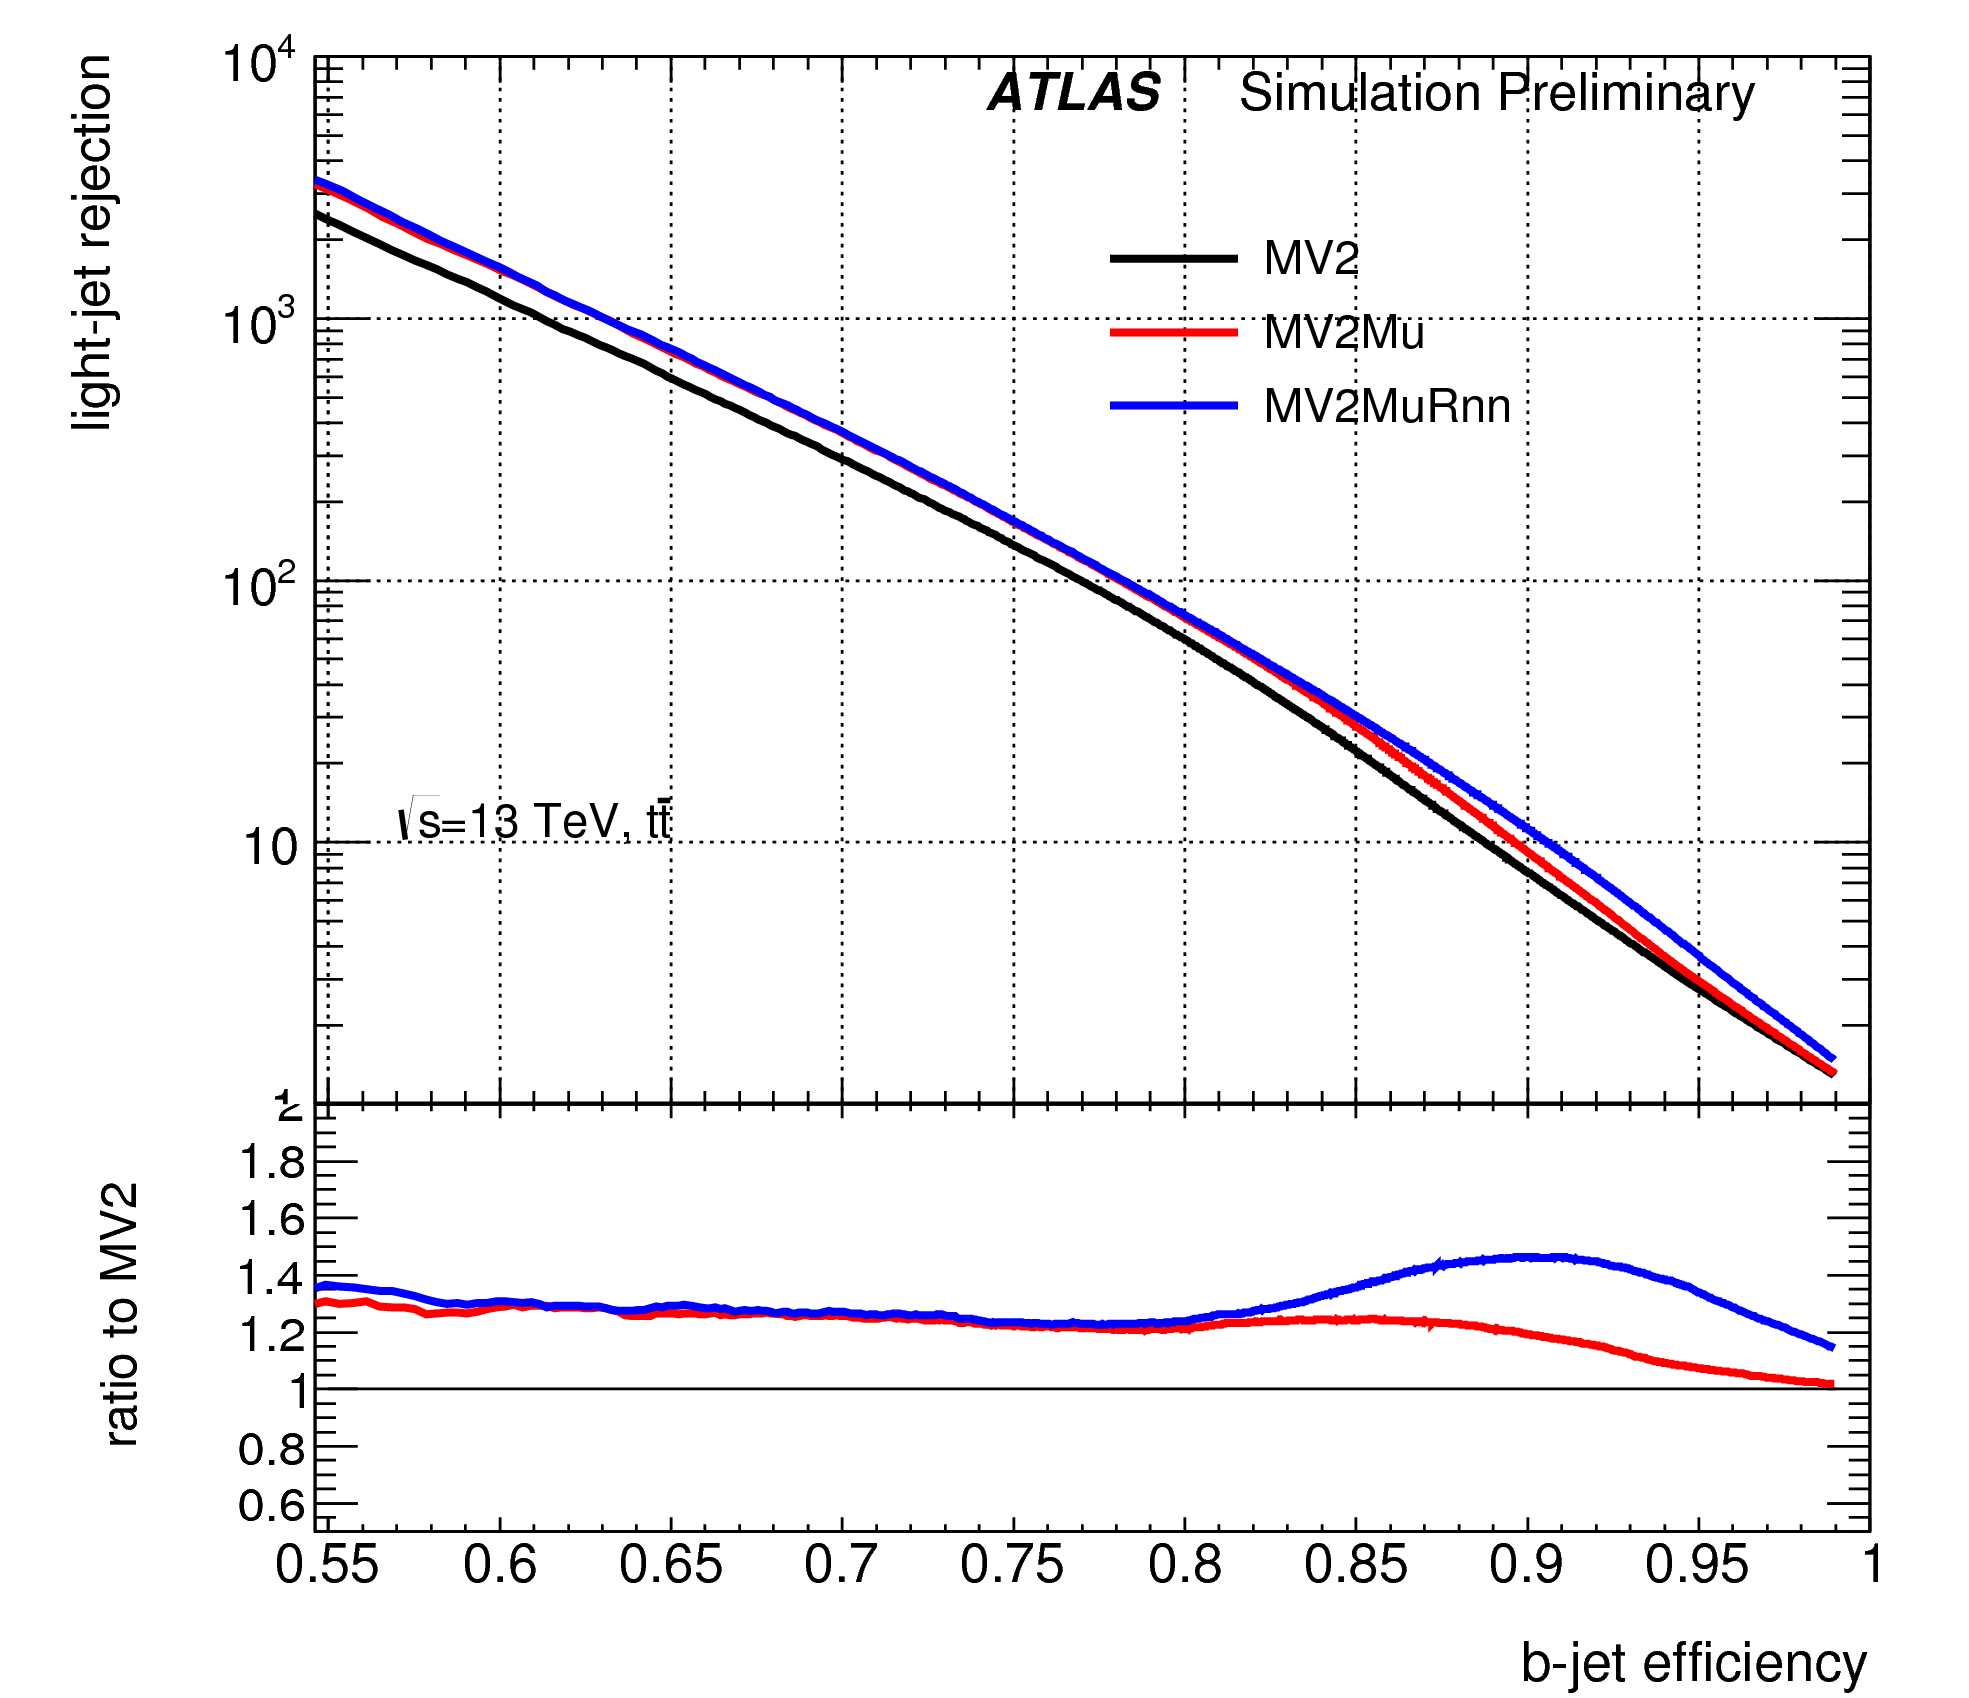
\includegraphics[width=0.48\textwidth]{figures/RNN/LRej_ttbar_combtagger.png}
 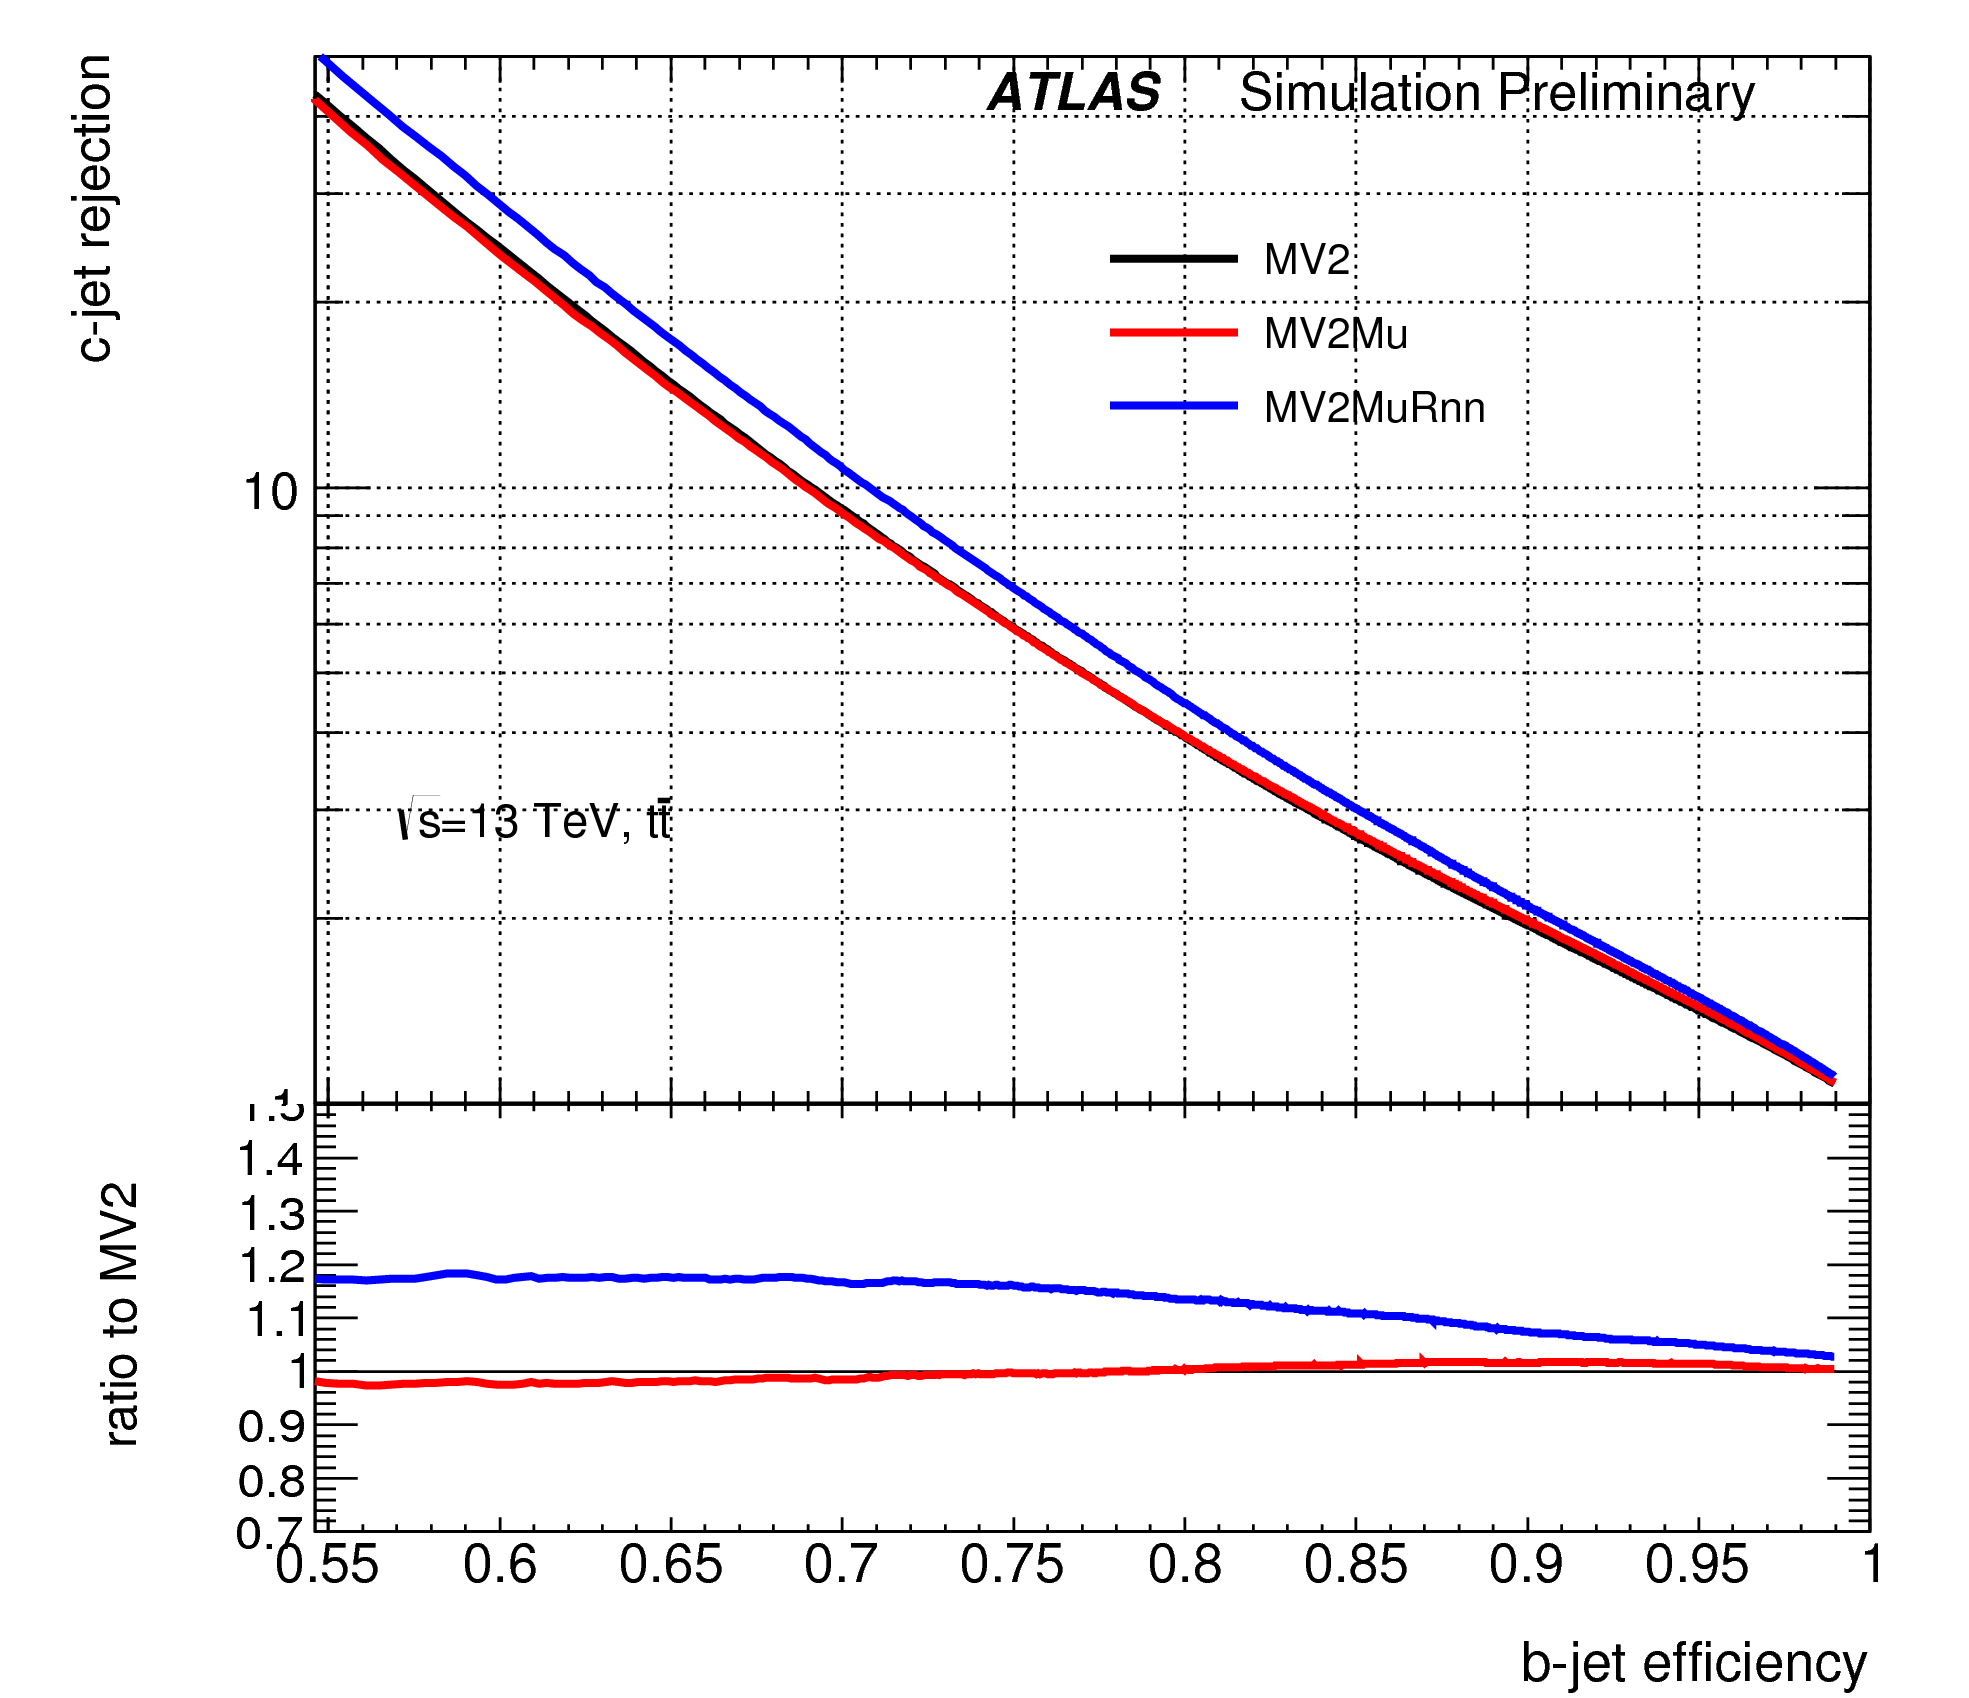
\includegraphics[width=0.48\textwidth]{figures/RNN/CRej_ttbar_combtagger.png}\\
 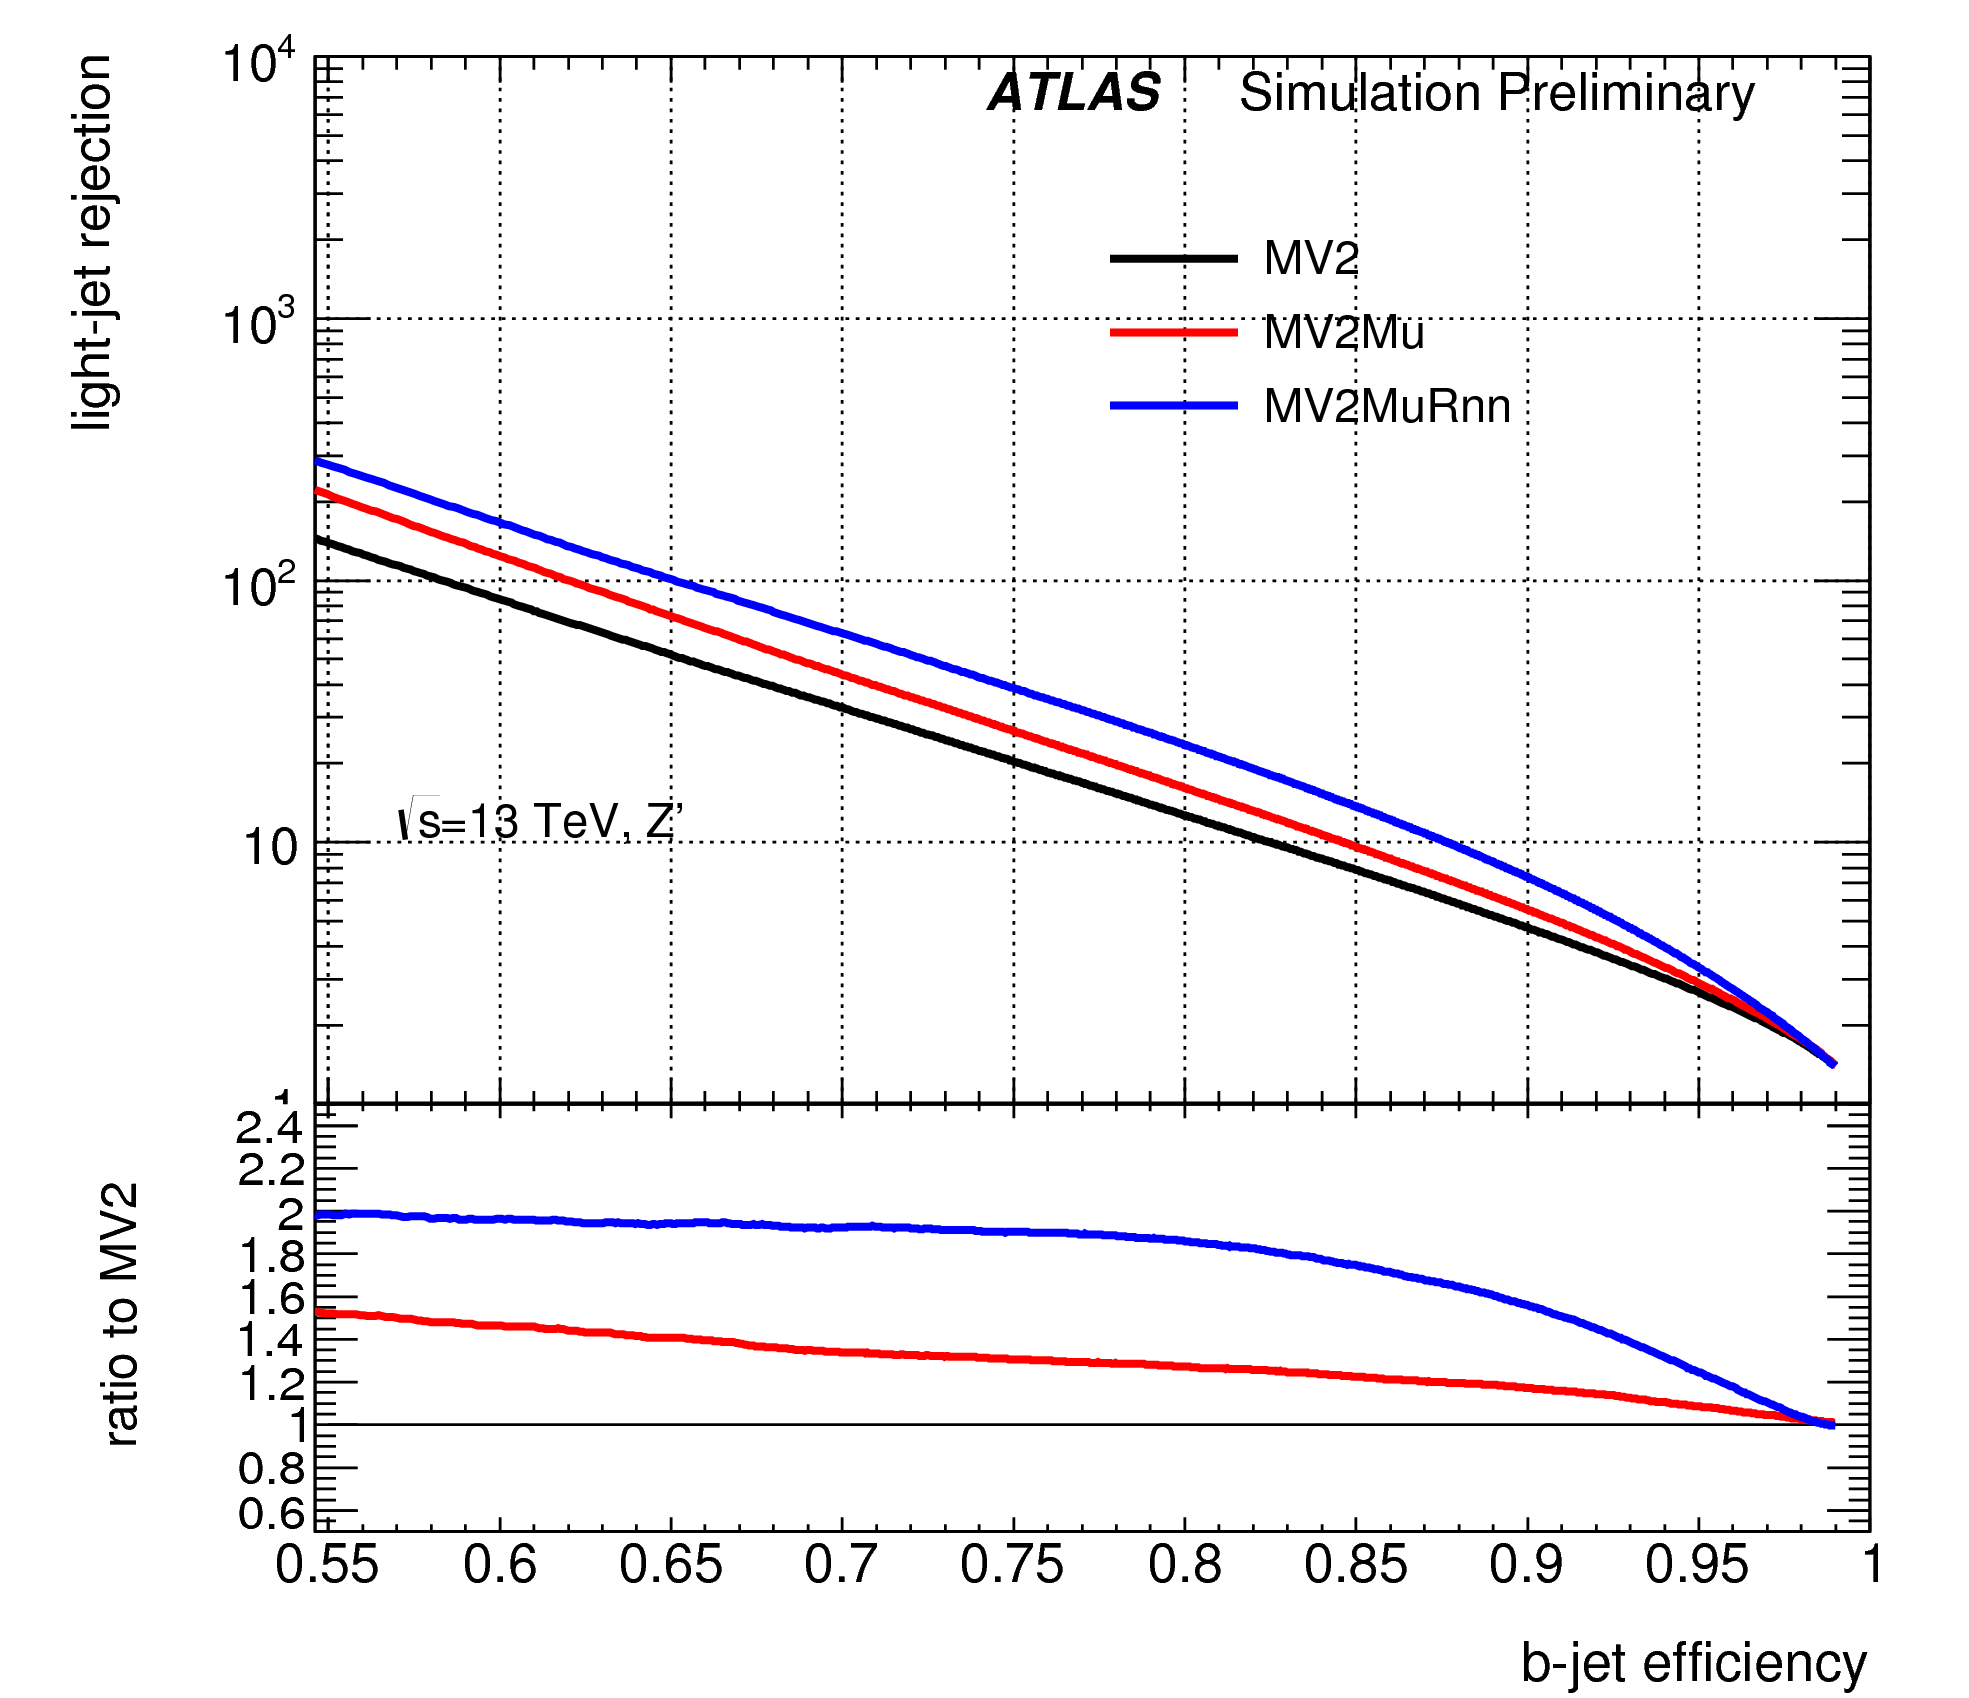
\includegraphics[width=0.48\textwidth]{figures/RNN/LRej_Zprime_combtagger.png}
 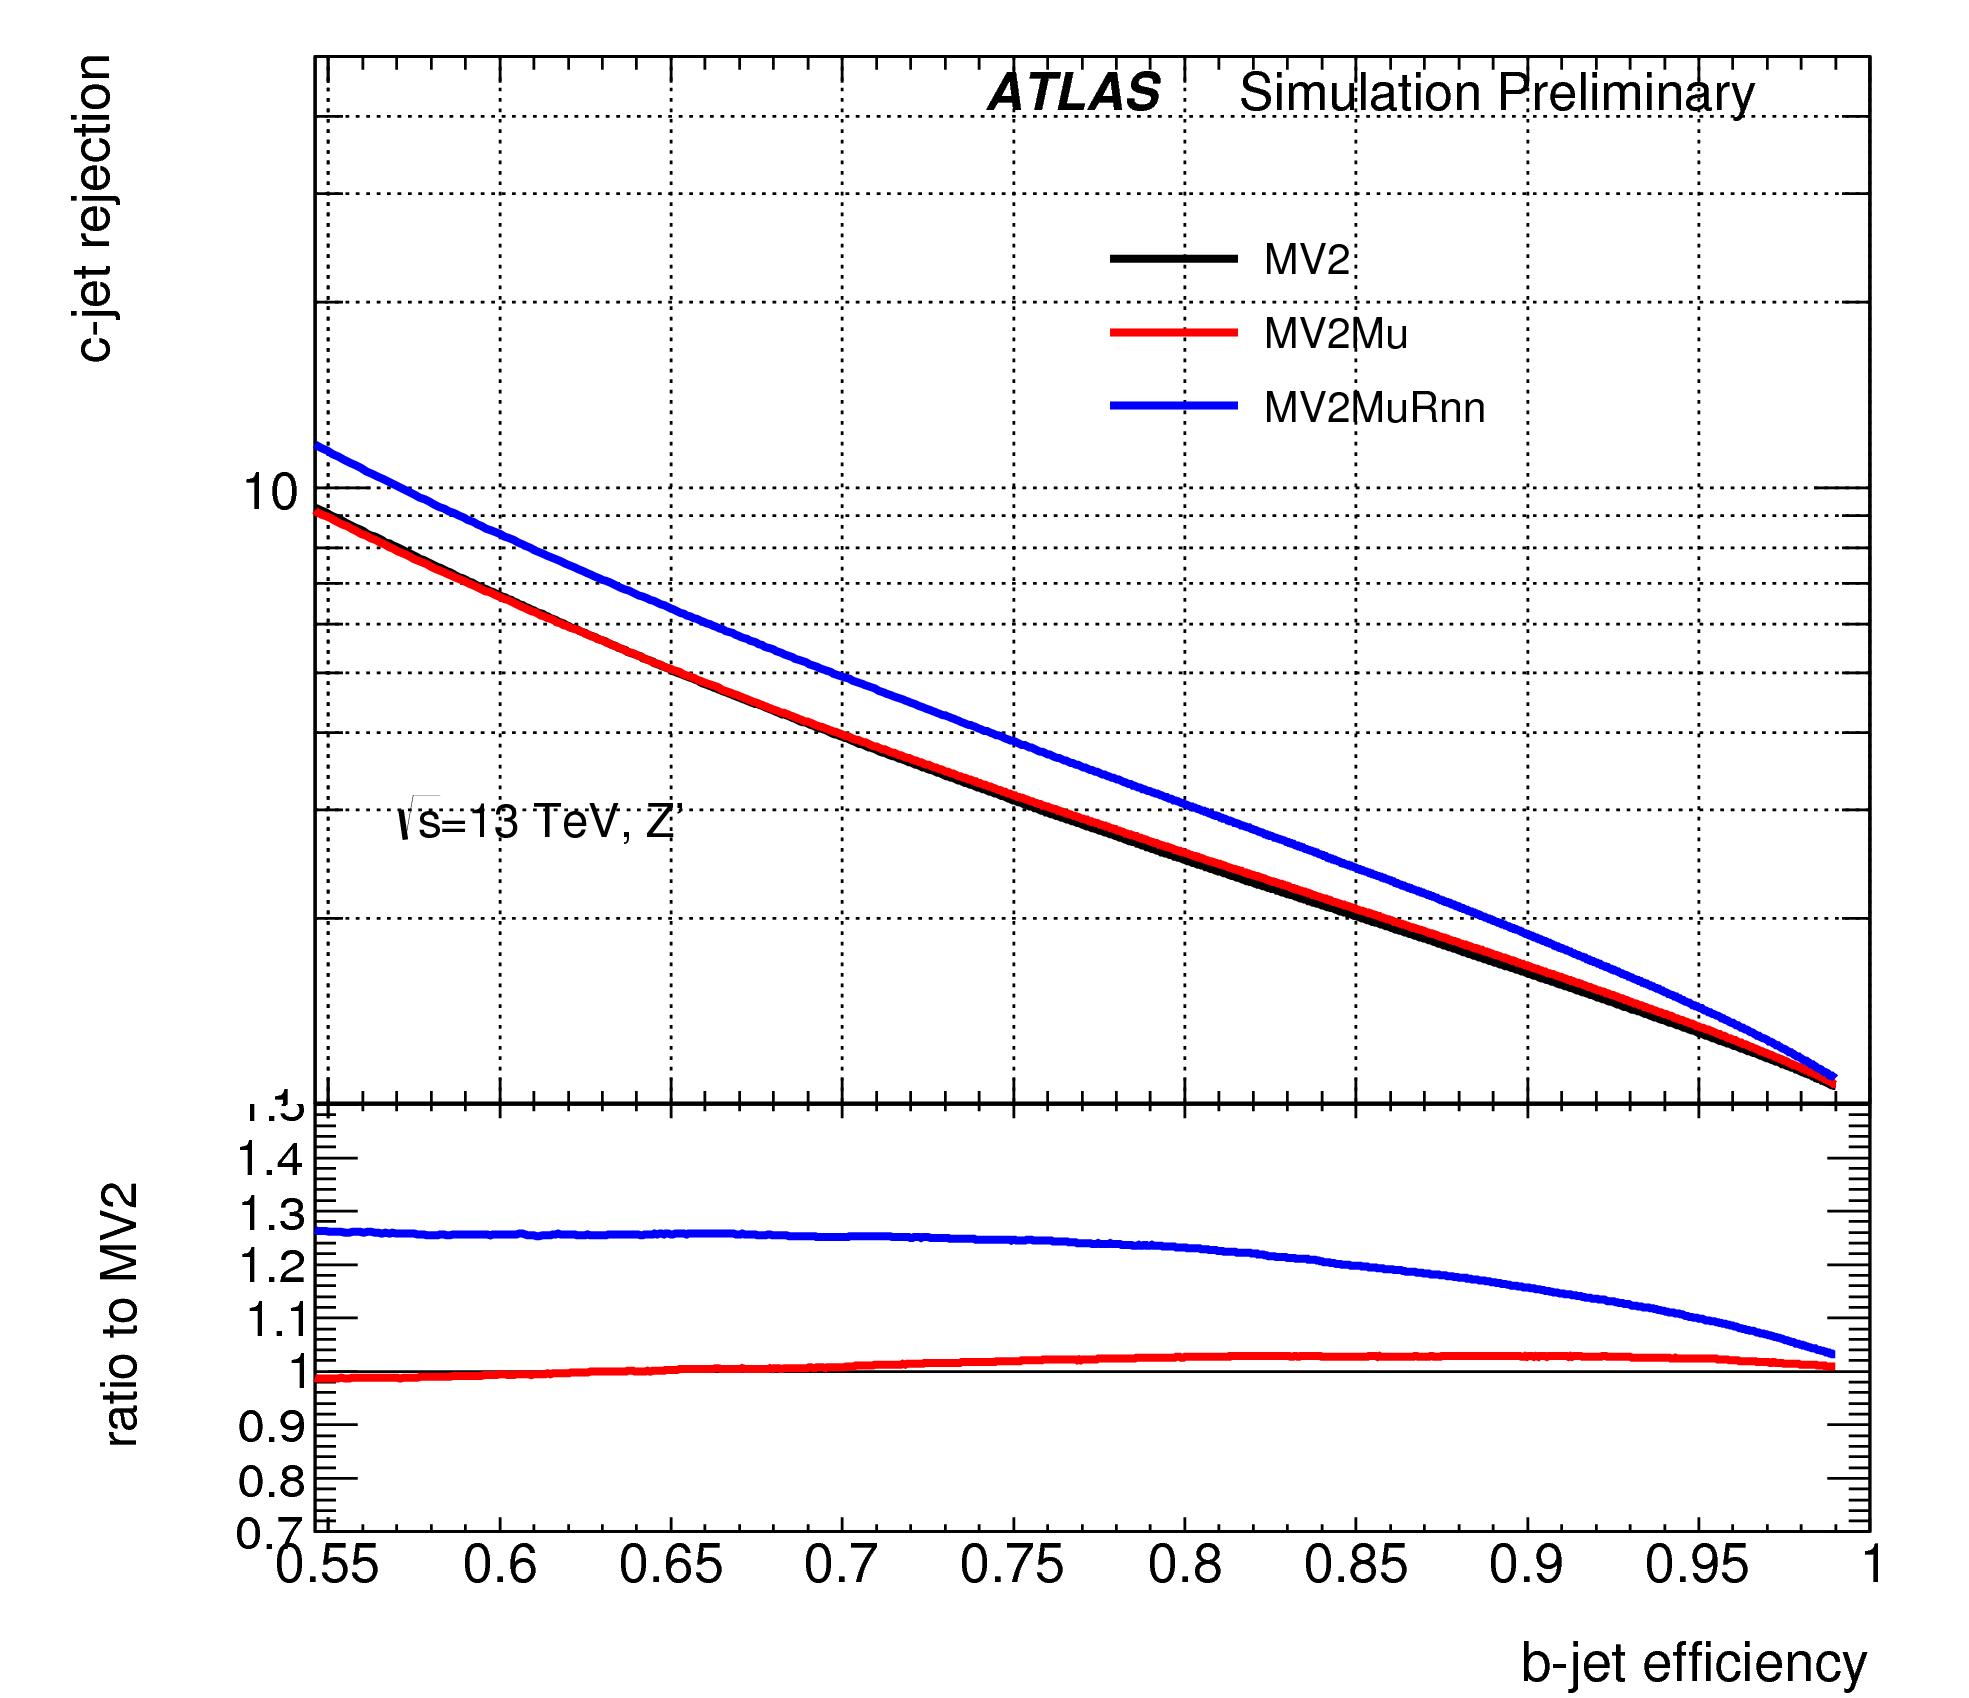
\includegraphics[width=0.48\textwidth]{figures/RNN/CRej_Zprime_combtagger.png}

 \caption{Light-flavor (left) and c-jet rejection (right) as a function of b-jet efficiency for \textit{MV2} (black line), \textit{MV2Mu} (red line), \textit{MV2MuRNN} (blue line). The algorithm evaluation is performed on $t\bar t$ (top) and Z' (botom) events. The ratio reported on the bottom of the figure is calculated for each \textit{MV2} variant (\textit{MV2Mu} and \textit{MV2MuRNN}) with respect to \textit{MV2}.}
  \label{fig:combtagger}
\end{figure}
